\chapter{Implementation}\label{chap:implementation}
%\section{Prototypes}
This section will describe the setup of the prototypes developed during this project.

\subsection{Prototype \#1}
\label{sec:implementation:prototypes:prototype1}
The first prototype was an Android phone application that showed the location of the user, the direction the phone was pointing, and the devices that were being pointed at.
The application used a $10 \times 10$ grid to simulate a square room in which the user and the devices to be controlled were located.
A set of imaginary devices was hardcoded into the application with fixed positions and the grid would look like the one shown in \Cref{table/prototype-grid}.
The user is positioned in the center at (5,5) by default. This position can be changed by using the \texttt{Up}, \texttt{Down}, \texttt{Left} and \texttt{Right} buttons.
When the user's direction changes a list of devices being pointed at is acquired by calculating the angle between the user's position and the position of each device.
The direction is found using magnetic fields such that $0$ is north, $-90$ is west, $90$ is east, etc. 
The angle between each smart device and the user is calculated finding the inverse tangent (arctangent) and then converting from radians to degrees such that we get:
\begin{equation}
\var{angle} = 180 / \pi * \arctan(\var{user.y} - \var{device.y} / \var{user.x} - \var{device.x})
\end{equation}
where \var{user.x} and \var{user.y} are the $x$ and $y$ coordinates of the user and likewise for the device.
A screenshot of this application is shown in \Cref{fig:prototype1-app-screenshots}.

% Thalley: Måske lave om et et Tikz coordinatsystem i stedet for? Fylder unødvendigt meget imo. 
\begin{table}[!htb] 
    \centering
    \tiny
    \begin{TAB}(e){|c:c:c:c:c:c:c:c:c:c|}{|c:c:c:c:c:c:c:c:c:c|}
     &  &  &  &  &  &  &  &  & Stereo \\
     &  &  &  &  &  &  &  &  &  \\
     &  &  &  &  &  & \begin{tabular}[c]{@{}l@{}}Coffee\\ Maker\end{tabular} &  &  &  \\ 
     &  &  &  &  &  &  &  &  &  \\ 
    \begin{tabular}[c]{@{}l@{}}Garage\\ Door\end{tabular} &  &  &  &  &  &  &  &  &  \\ 
     &  & Lamp 2 &  &  &  &  &  &  &  \\
     &  &  &  &  &  &  &  &  &  \\ 
     &  &  &  &  &  &  &  &  &  \\ 
     &  &  &  &  &  &  &  &  &  \\ 
    Lamp 1 &  &  &  &  & TV &  &  &  &  \\
    \end{TAB}    
    \caption{Grid showing the position of devices. Lamp 1 is located at (0,0) and Stereo is located at (9,9)}
    \label{table/prototype-grid}
\end{table}

\begin{figure}[!htb]%
    \centering
    \subfloat{
        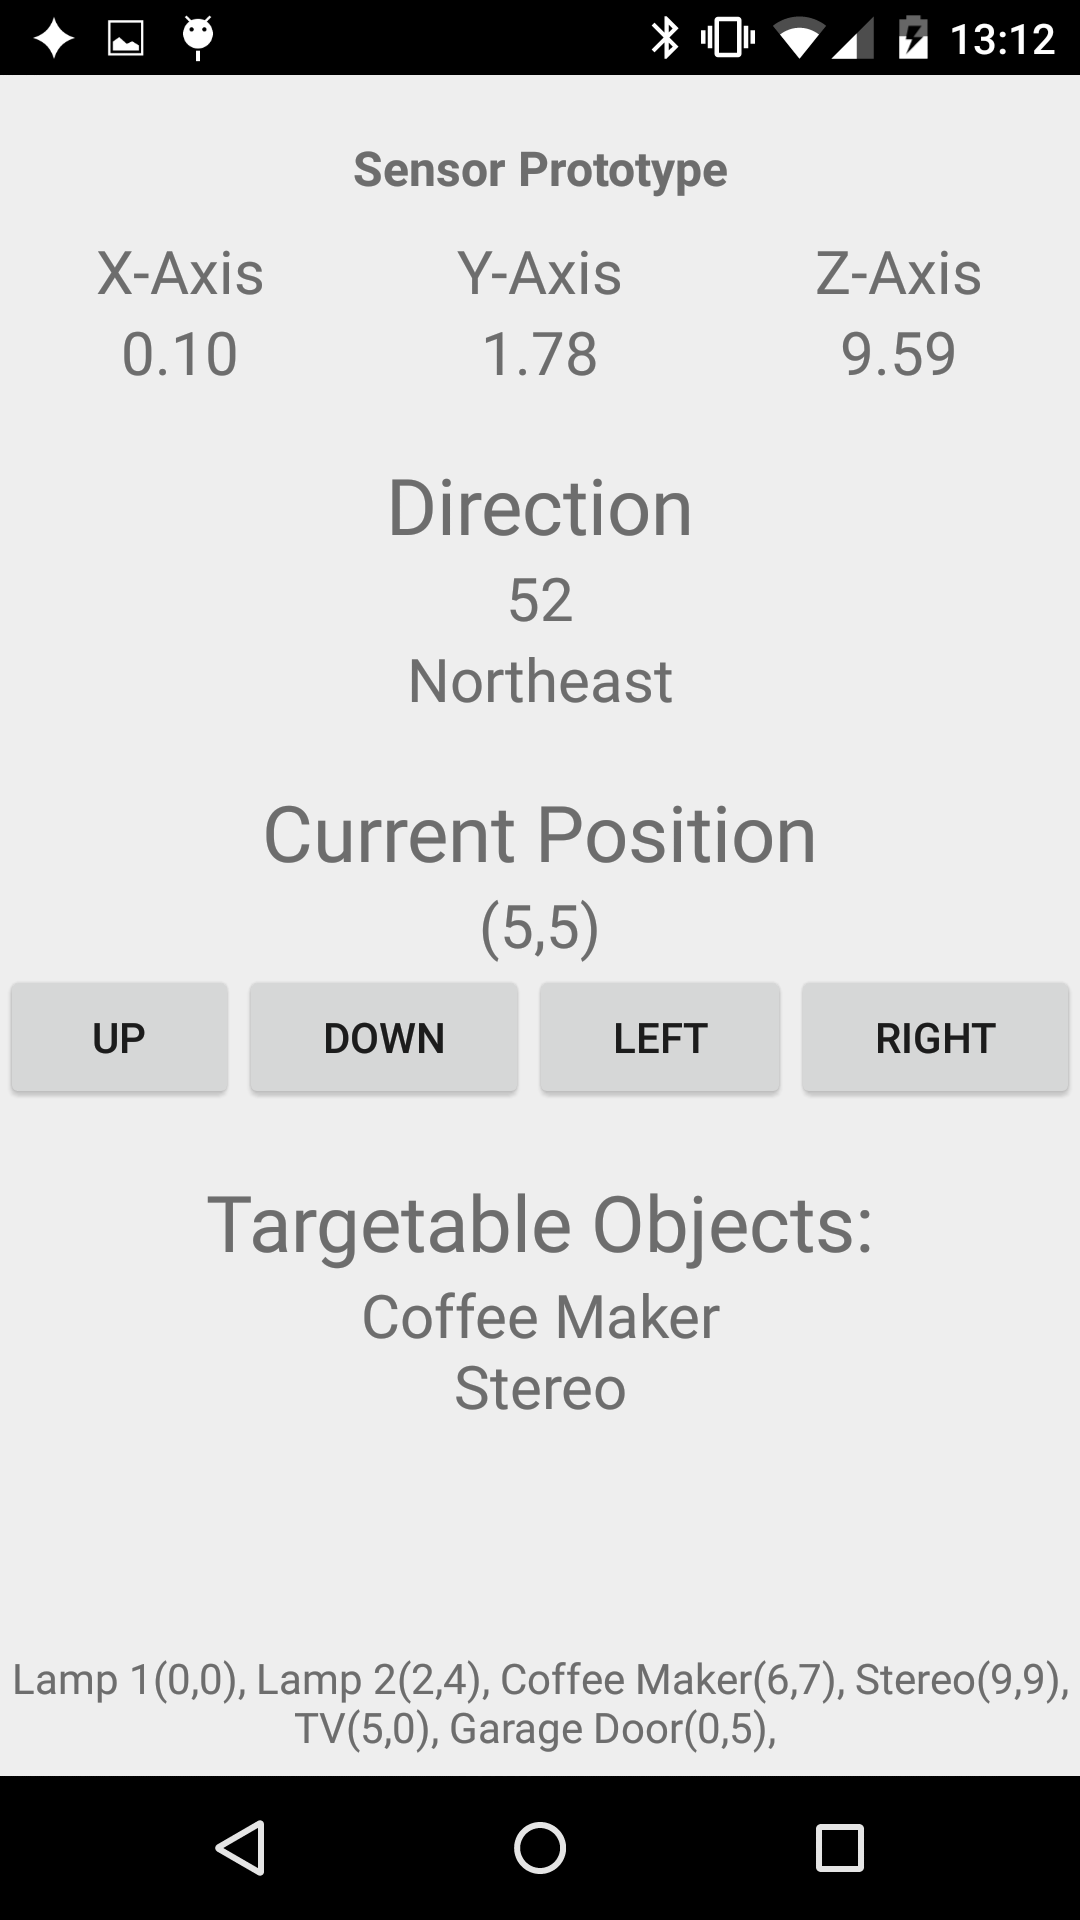
\includegraphics[width=0.3\textwidth]{images/Prototype1_Android_1.png}
    }
    \subfloat{
        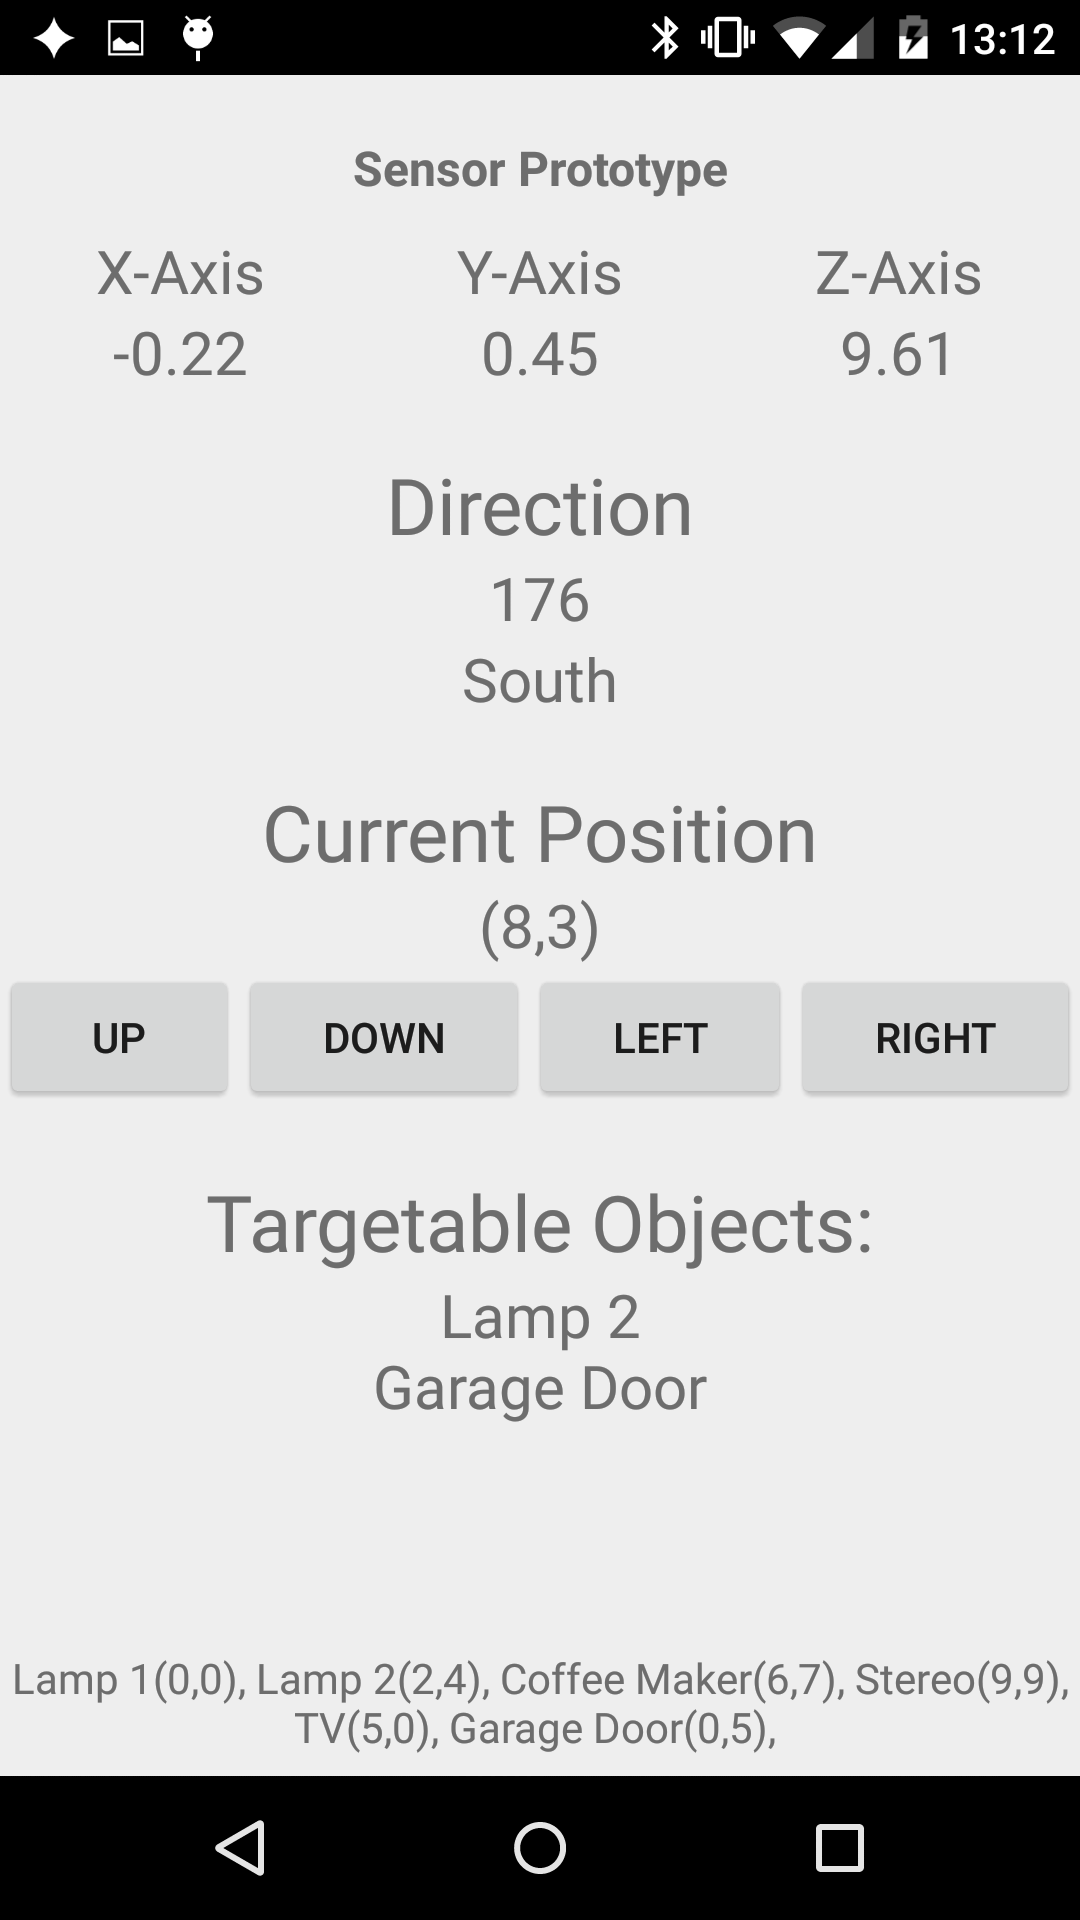
\includegraphics[width=0.3\textwidth]{images/Prototype1_Android_2.png}
    }
    \caption{Screenshots of the first prototype.}
    \label{fig:prototype1-app-screenshots}
\end{figure}


\subsection{Prototype \#2}
\label{sec:implementation:prototypes:prototype2}

The second prototype consisted of an iOS application similar to the Android application described in section \ref{sec:implementation:prototypes:prototype1} and a server that represented two controllable lamps.
The platform was changed from Android to iOS because the application would later use Estimote beacons and there was no Android Indoor Location SDK available for this. 

\subsubsection{Major Changes}
\begin{itemize}
    \item Introduction of a server for the application to interact with.
    \item Switched platform from Android to iOS.
\end{itemize}

In this prototype the room is still represented as a grid and the user is placed in the center of the grid, however the user is unable to change position.
This is because the first prototype showcased the idea of pointing at devices from different locations sufficiently and the next step would be to use the actual location of a user using Estimote beacons.
As shown in \Cref{fig:prototype2-app-screenshots} the user can see his direction as an angle between himself and north.
Devices are represented as orange dots and if the user points towards one of them two buttons will appear that allow the user to interact with the device by either turning it \texttt{on} or \texttt{off}.
When the user turns a device on or off, it will be reflected on the server, 
where a corresponding box will have the color \texttt{green} when turned on and \texttt{red} when turned off as shown in \Cref{fig:prototype2-server-screenshot}.

\begin{figure}[!htb]%
    \centering
    \subfloat{
        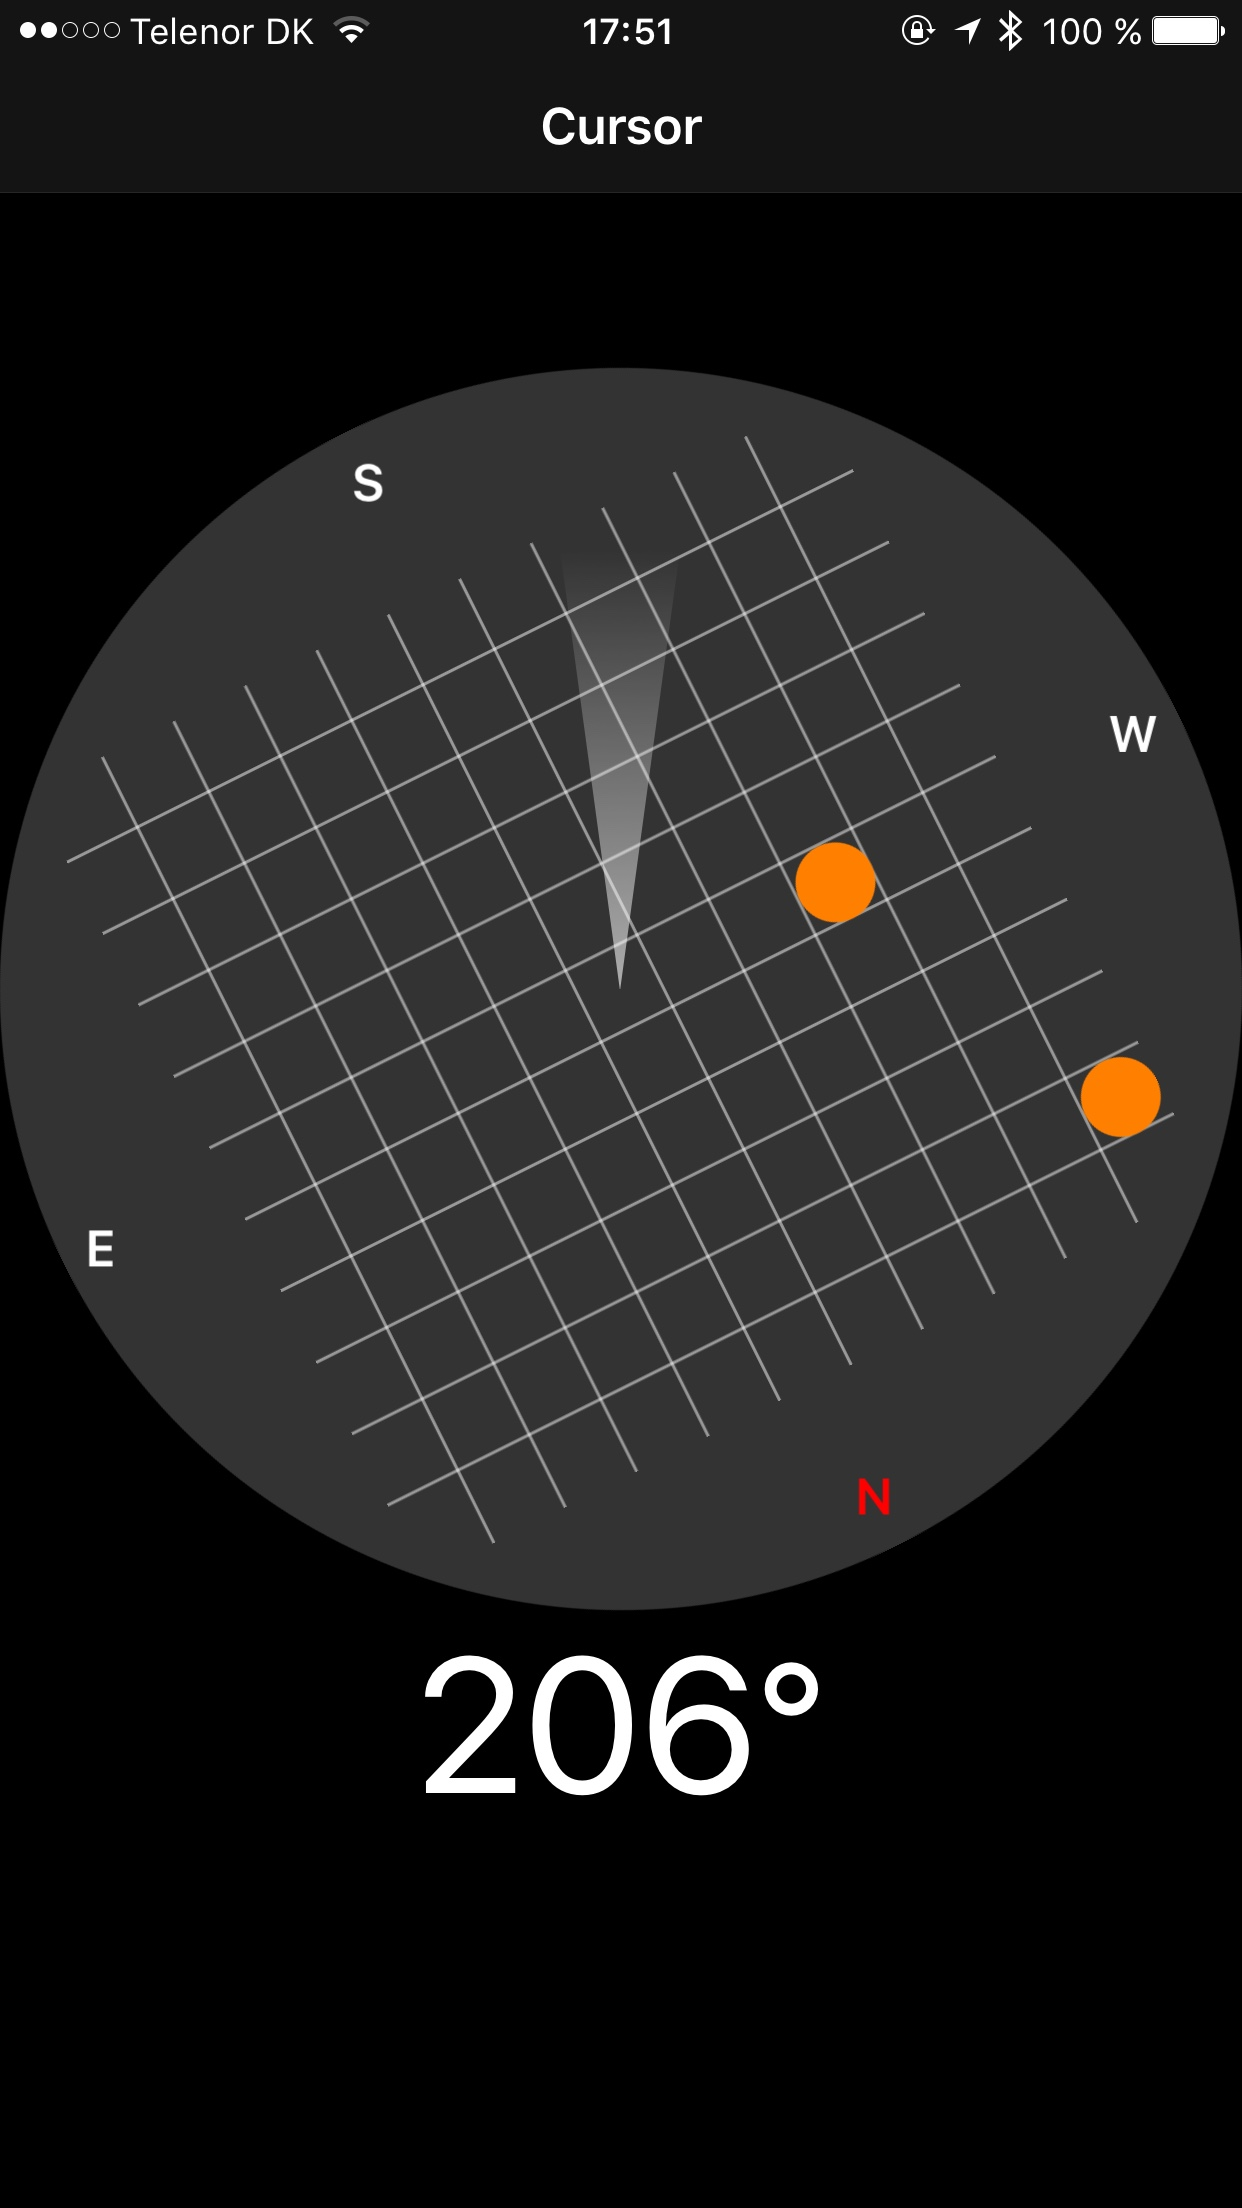
\includegraphics[width=0.3\textwidth]{images/Prototype2_iOS_1.png}
    }
    \subfloat{
        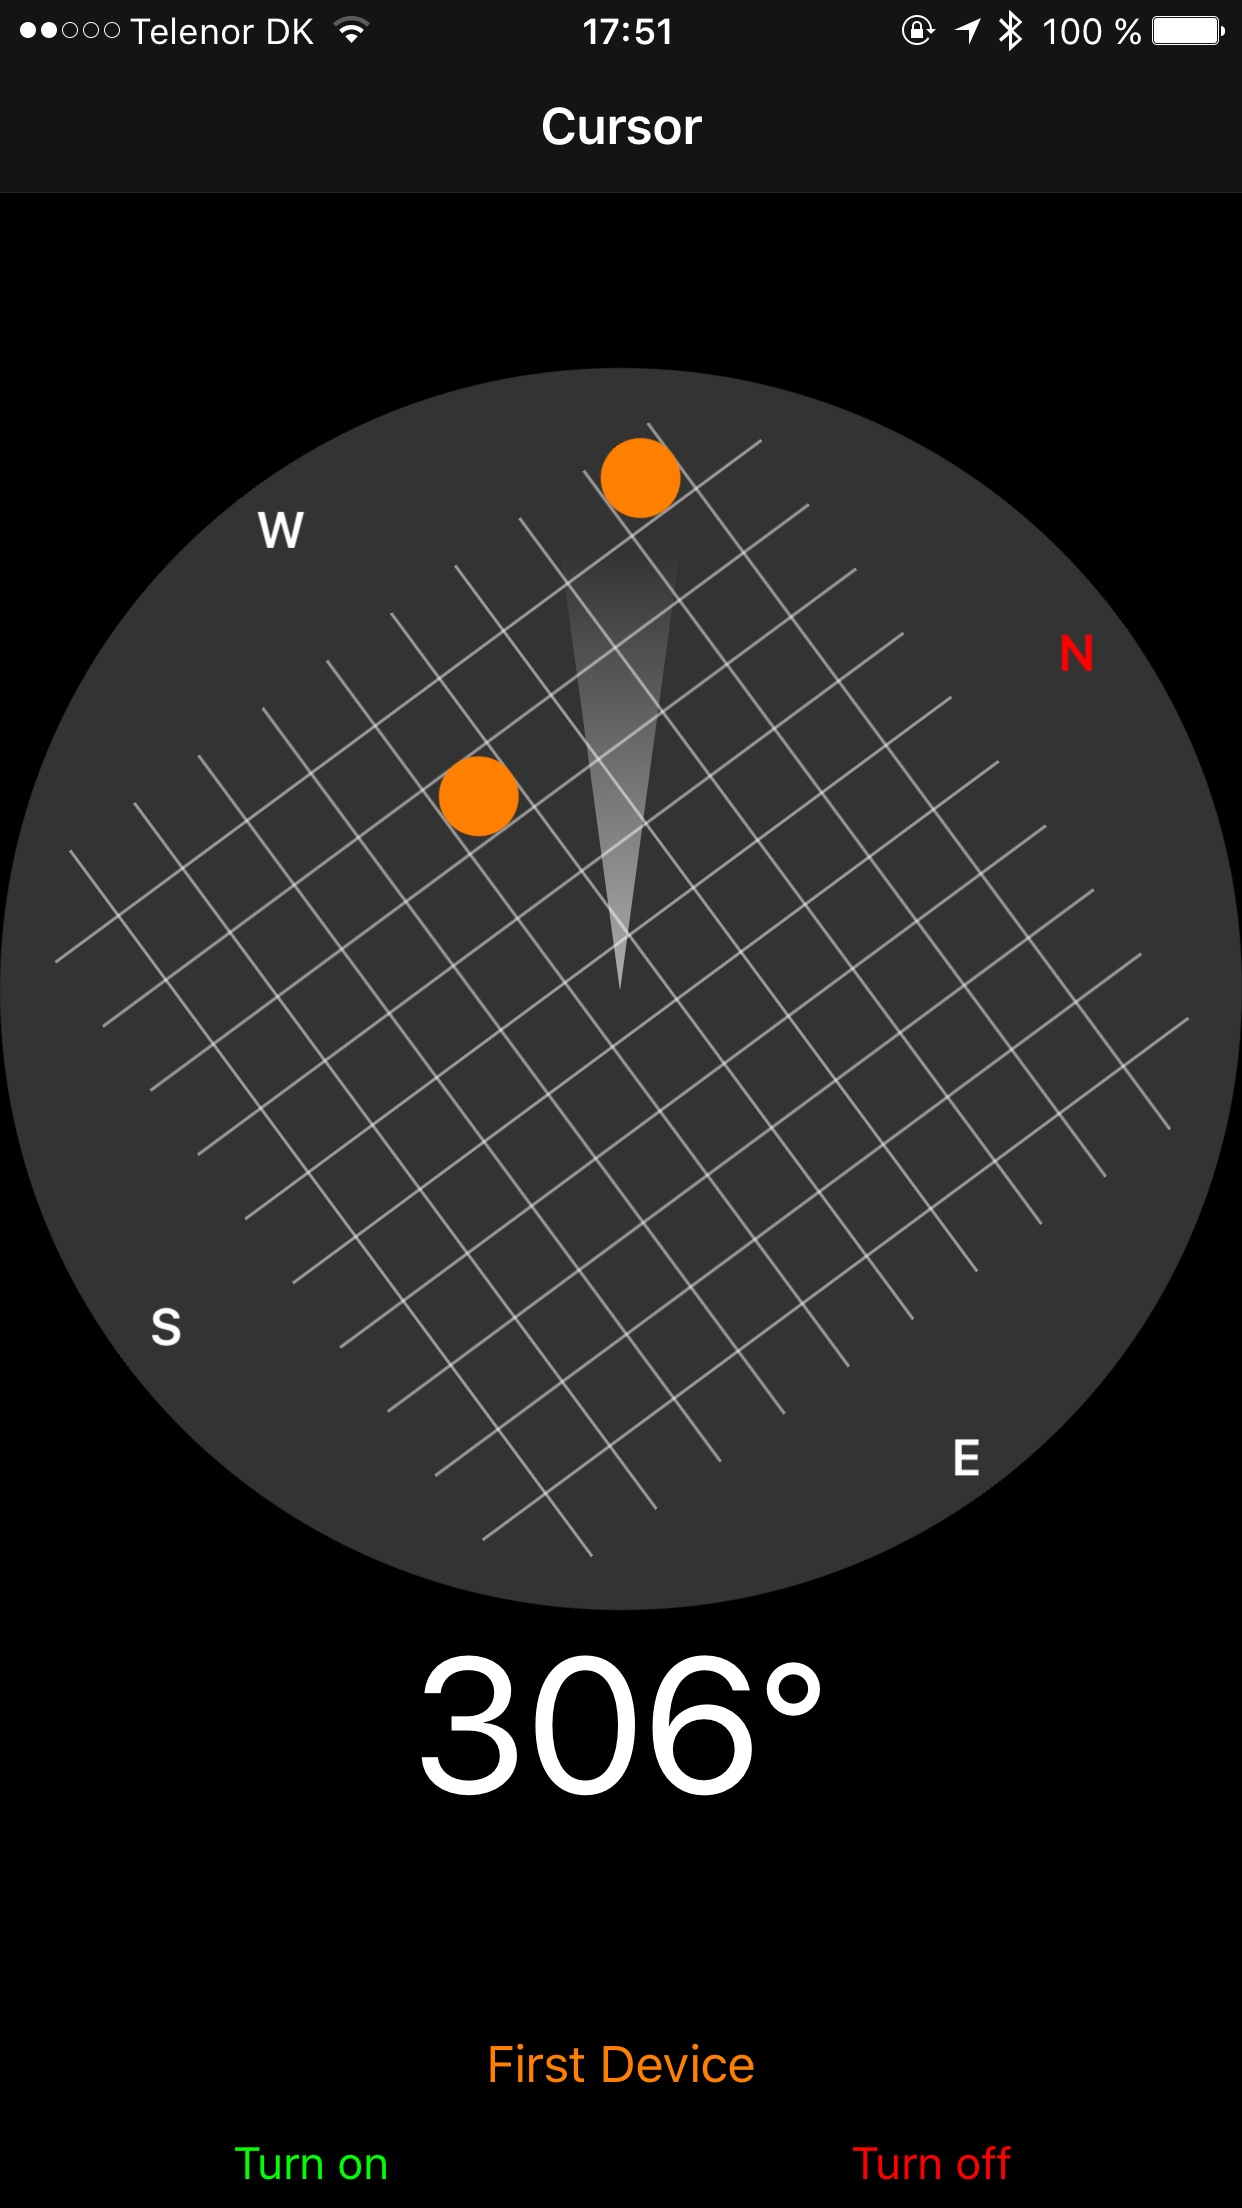
\includegraphics[width=0.3\textwidth]{images/Prototype2_iOS_2.png}
    }
    \caption{Screenshots of the second prototype application.}
    \label{fig:prototype2-app-screenshots}
\end{figure}

\begin{figure}[!htb]
    \centering
    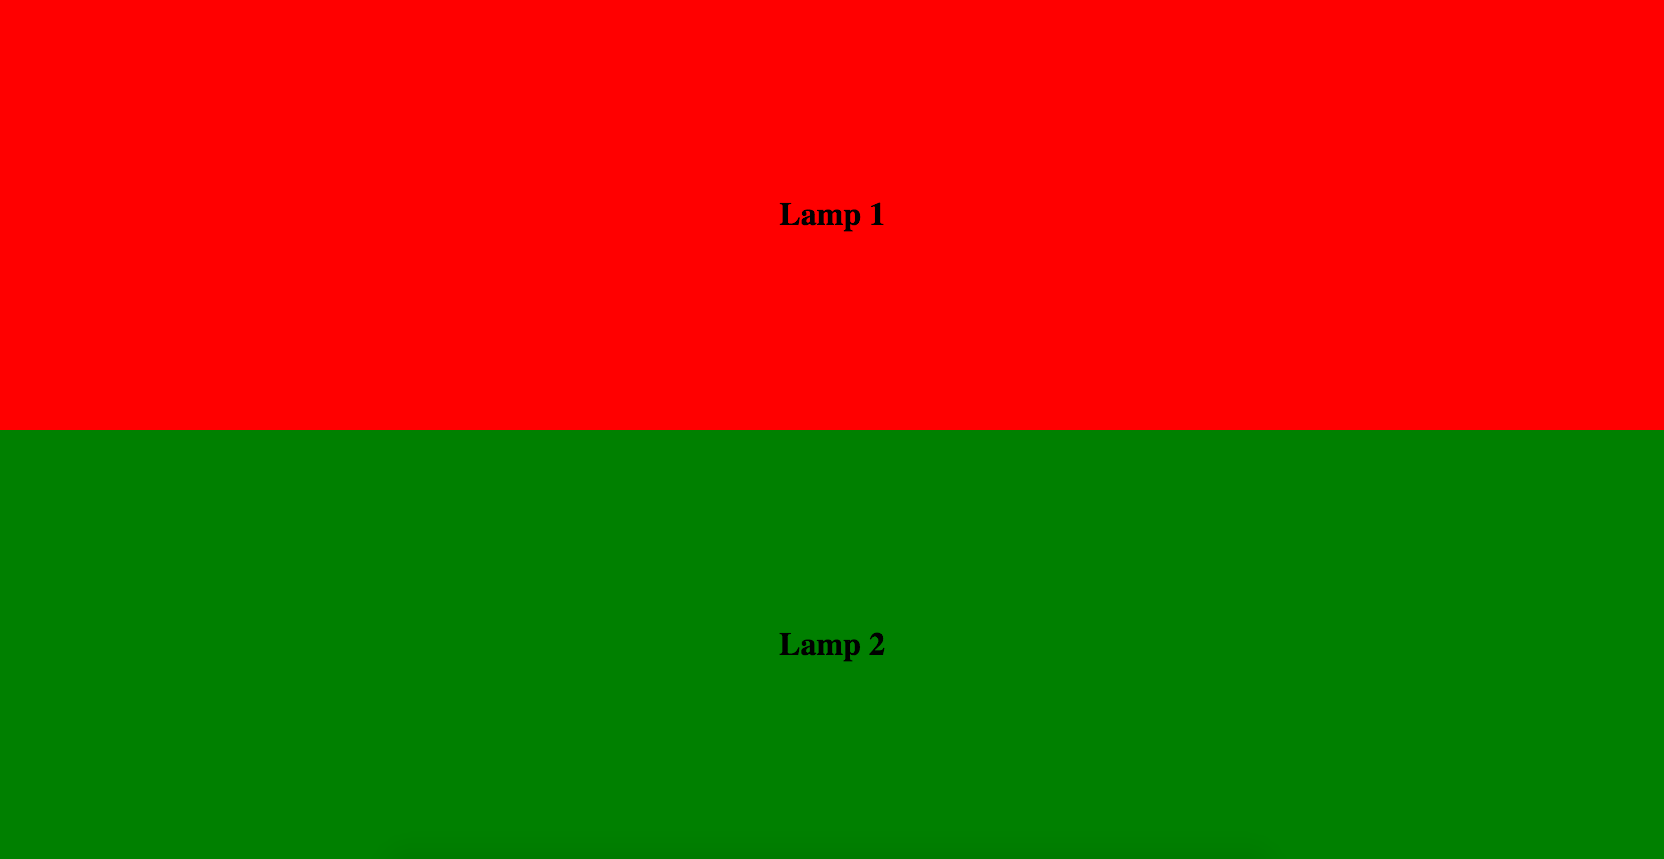
\includegraphics[scale=0.2]{images/Prototype2_Server.png}
    \caption[caption]{Screenshot of the server representing two lamps in the second prototype.\\\texttt{Green}: On, \texttt{Red}: Off}
    \label{fig:prototype2-server-screenshot}
\end{figure}

\subsection{Prototype \#3}
\label{sec:implementation:prototypes:prototype3}

The third prototype builds upon the second prototype for iOS which was expanded to include some new features. The second prototype would assume that the user was positioned in the center of the room but the new prototype takes the users position into account when determining devices being pointed at. Estimote iBeacons and the SDK provided by Estimote for indoor positiong was utilized in order to determine the position of the user.

The indoor SDK from Estimote provides a visualization of the room in which the positioning takes place as well as a visualization of the installed beacons and the position of the user. The view can be used to visualize custom objects. Figure \ref{fig:prototype3-room-screenshot} shows two red circles in the room. Each of the circles represent one of the virtual lamps introduced in the second prototype. The color of the lamp indicate the state the lamp is in. A lamp can either be on or off. The states are represented by red and green respectively.

Furthermore the prototype added support for training and recognizing gestures using the ThreeDollarGesture library. Users can add a gesture by giving the gesture a name and train it at least five times. When added, the gesture can be used when poiting at a lamp to toggle the state of the lamp. For example, if the user has trained a circle named ``Half Circle'', he can visit the screen showing his lamps and his position, point at one or more lamps and perform the ``Half Circle'' gesture in order to either turn on or turn off the lamps.

The third prototype does not support associating a gesture with an action, that is, perform a specific action for a specific gesture. Nor does it support creating a model of a room. The prototype is limited to a specific room modelled after the living room of one of the research members.

\subsubsection{Major Changes}
\begin{itemize}
\item Uses iBeacons to position the user in a room and take his position into account when determining devices being pointed at.
\item Adds training and recognition of gestures in order to trigger actions of a controllable device.
\item Adds a graphical representation of the room in which the beacons and the devices are installed.
\end{itemize}

\begin{figure}[!htb]%
    \centering
    \subfloat{
        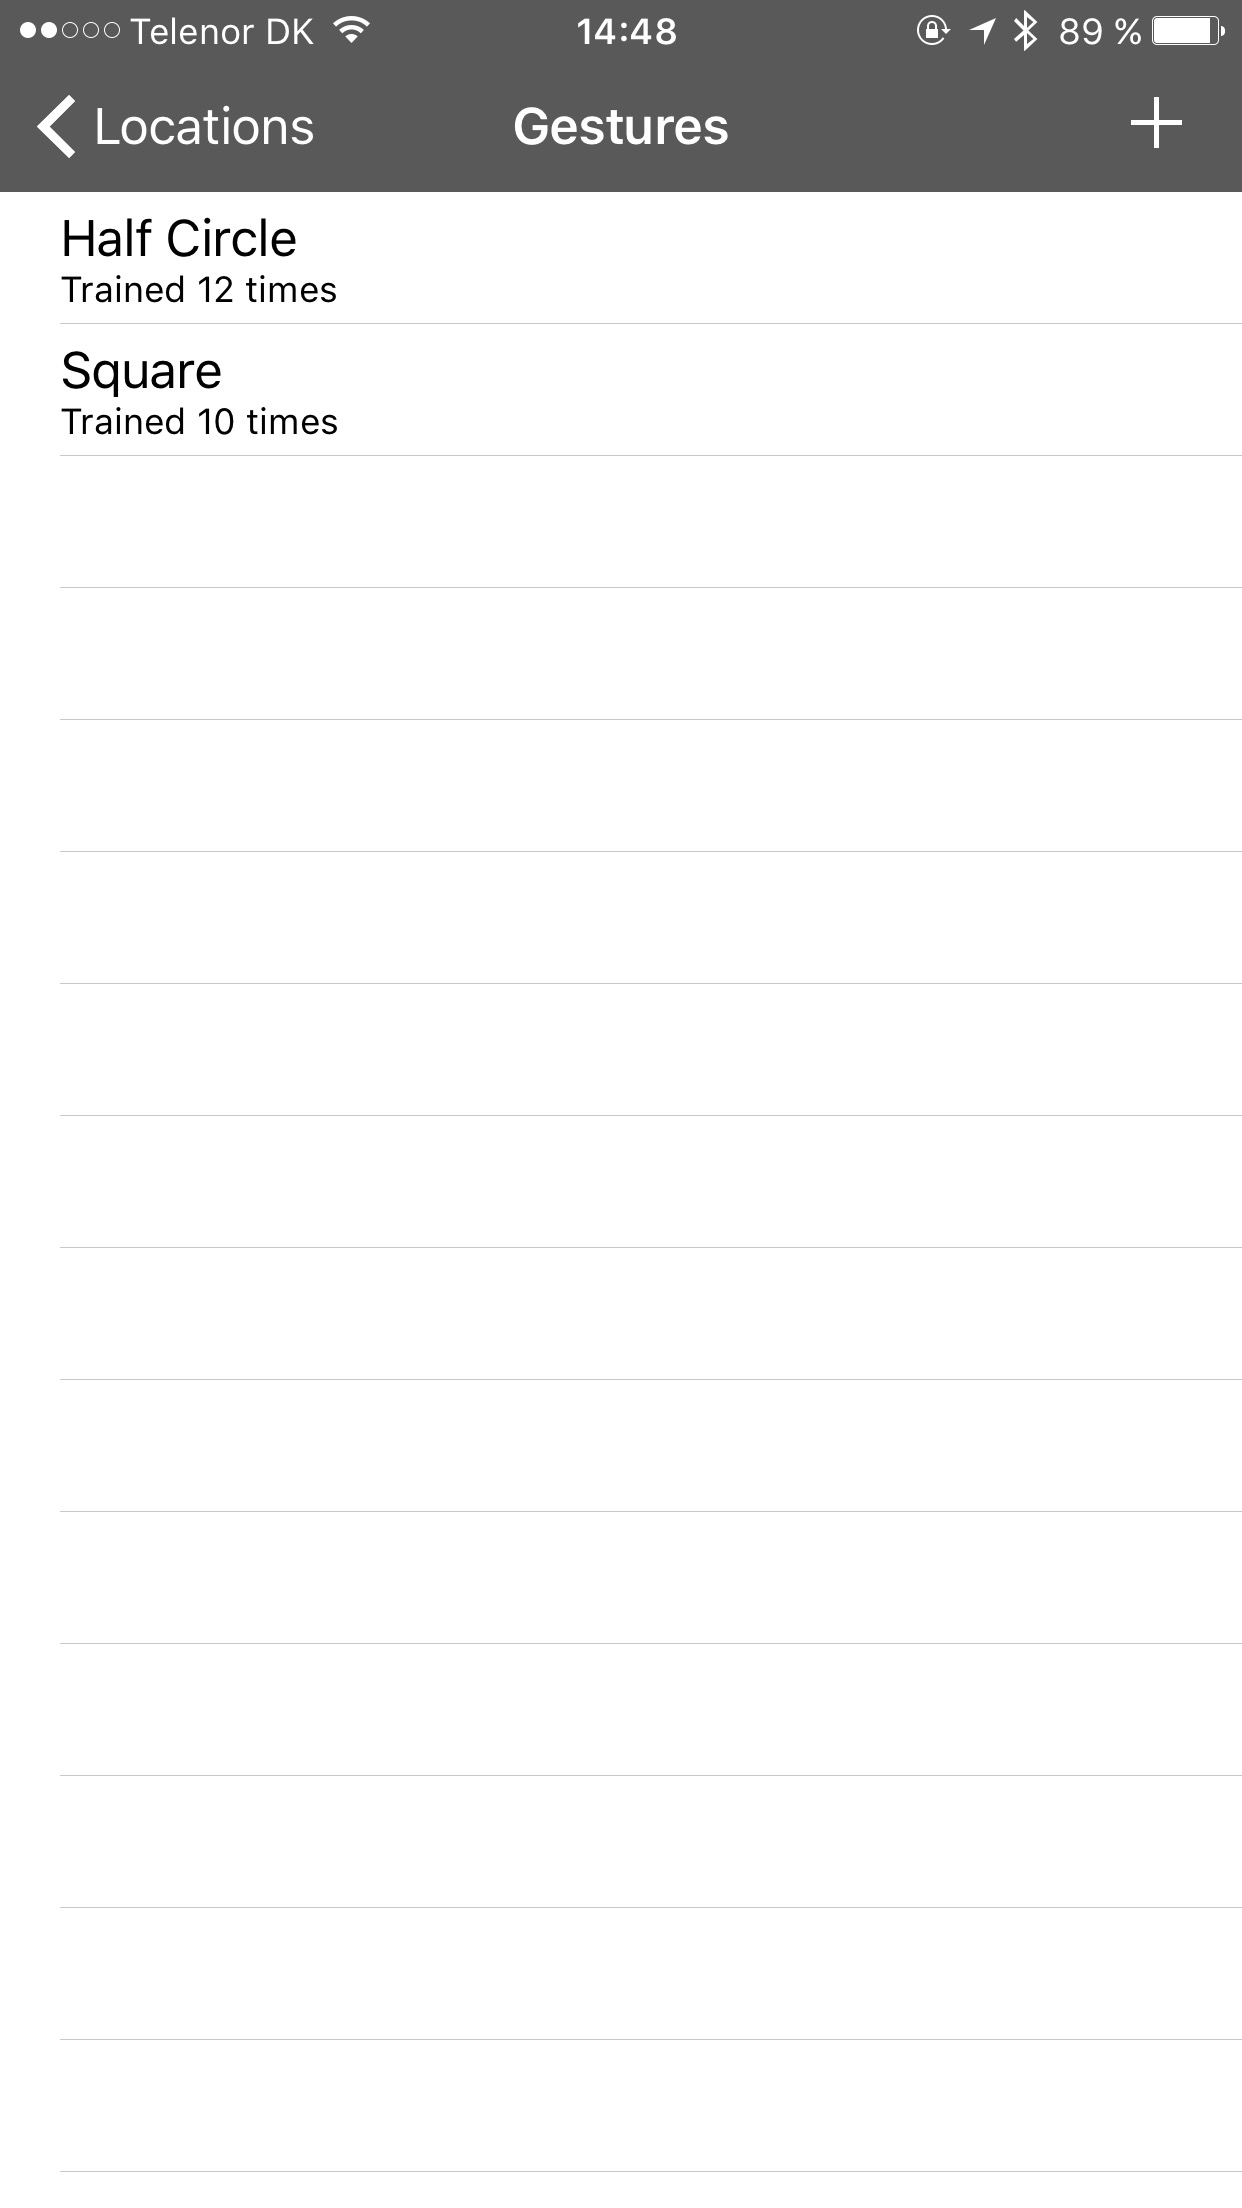
\includegraphics[width=0.3\textwidth]{images/prototype-3-all-gestures}
    }
    \subfloat{
        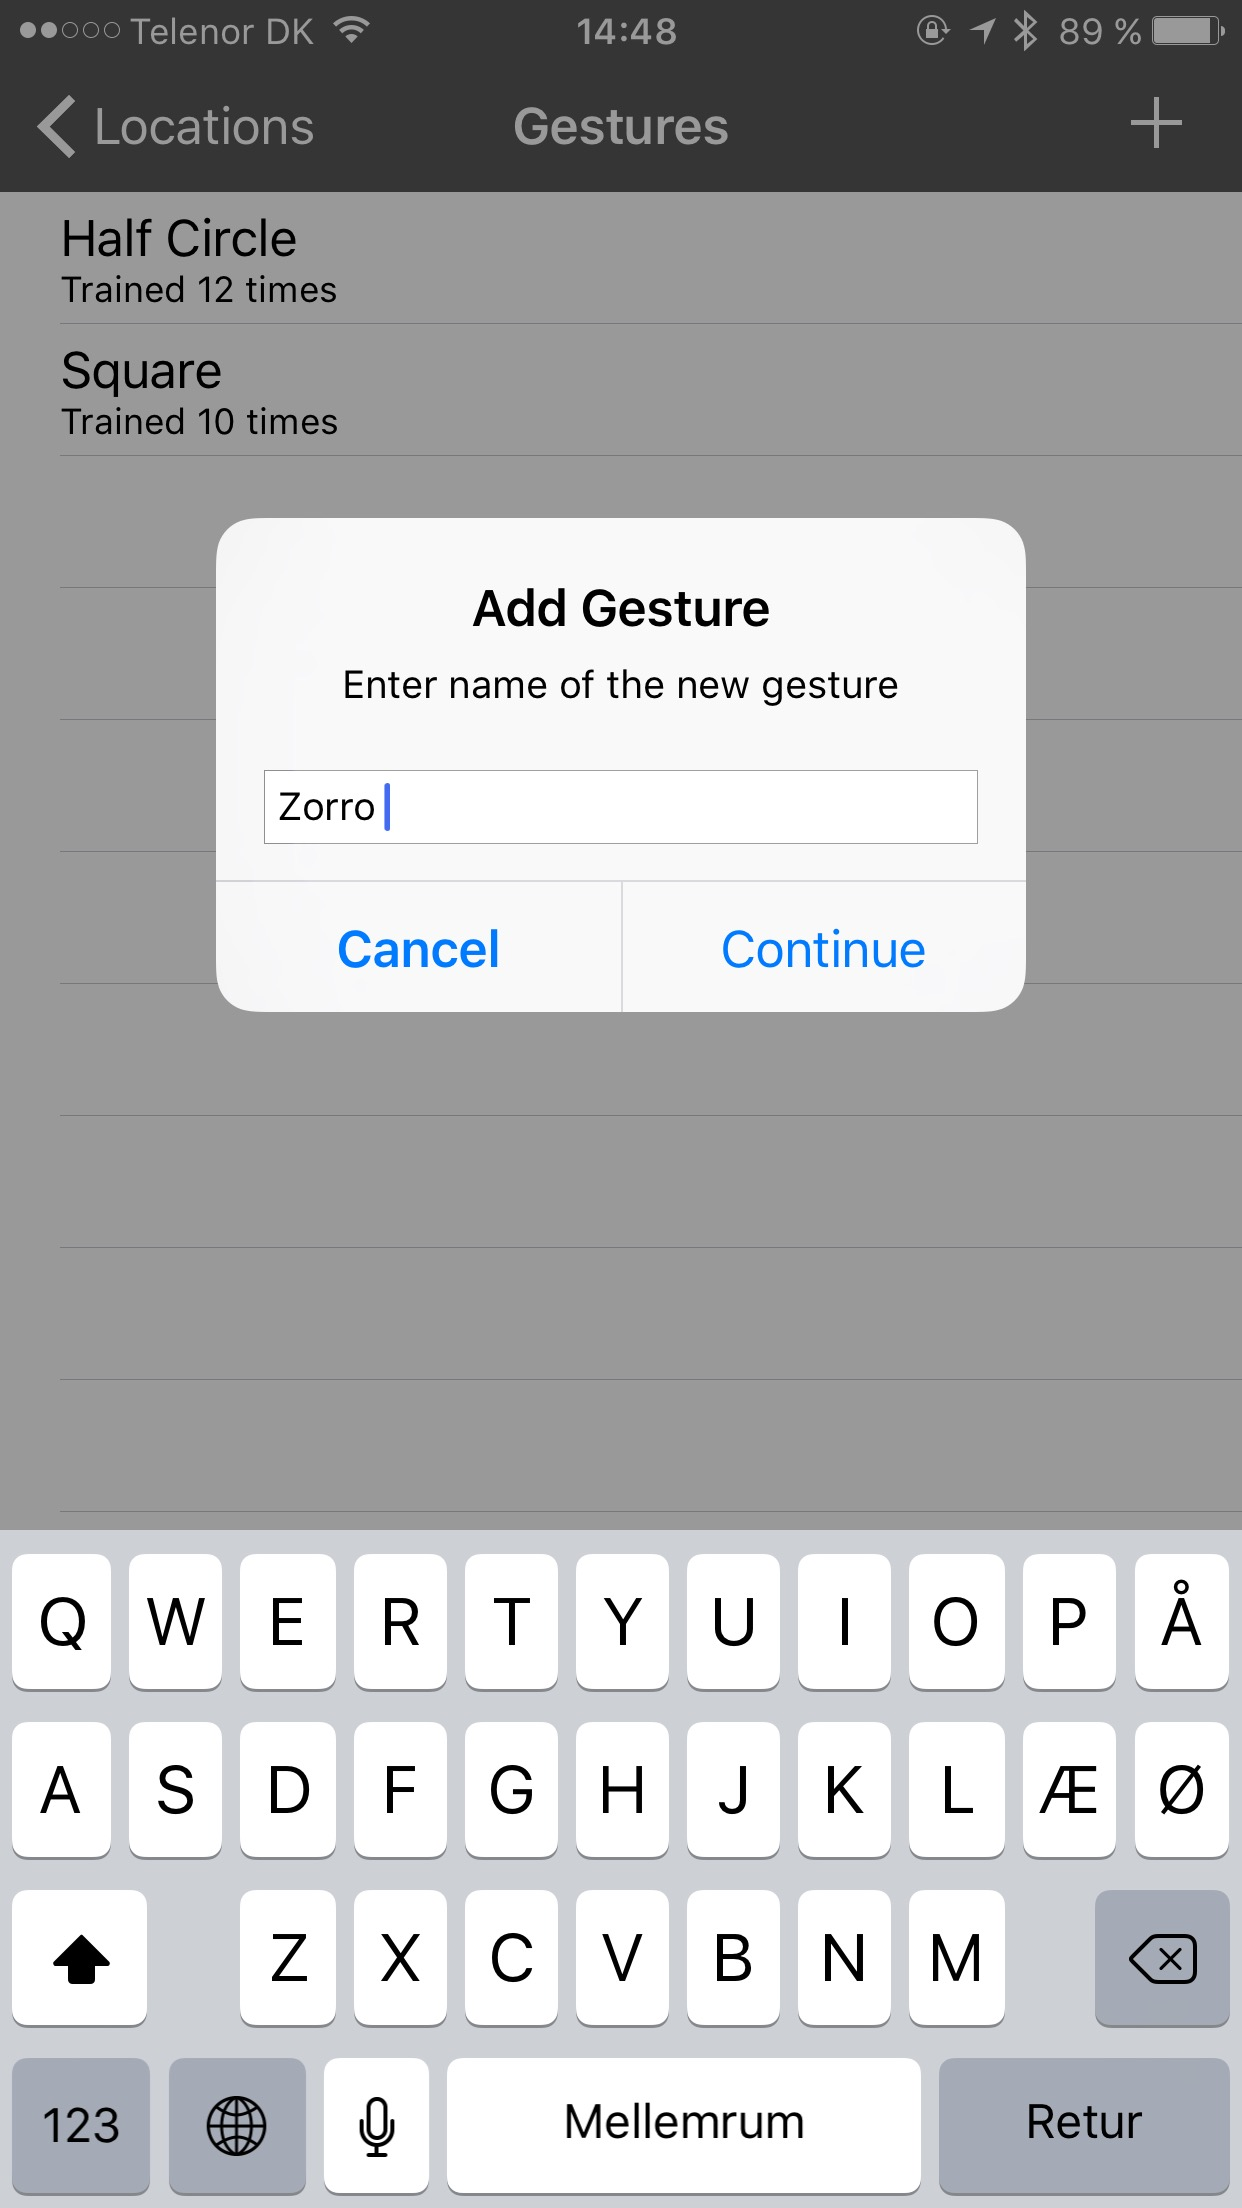
\includegraphics[width=0.3\textwidth]{images/prototype-3-new-gesture}
    }
    \subfloat{
        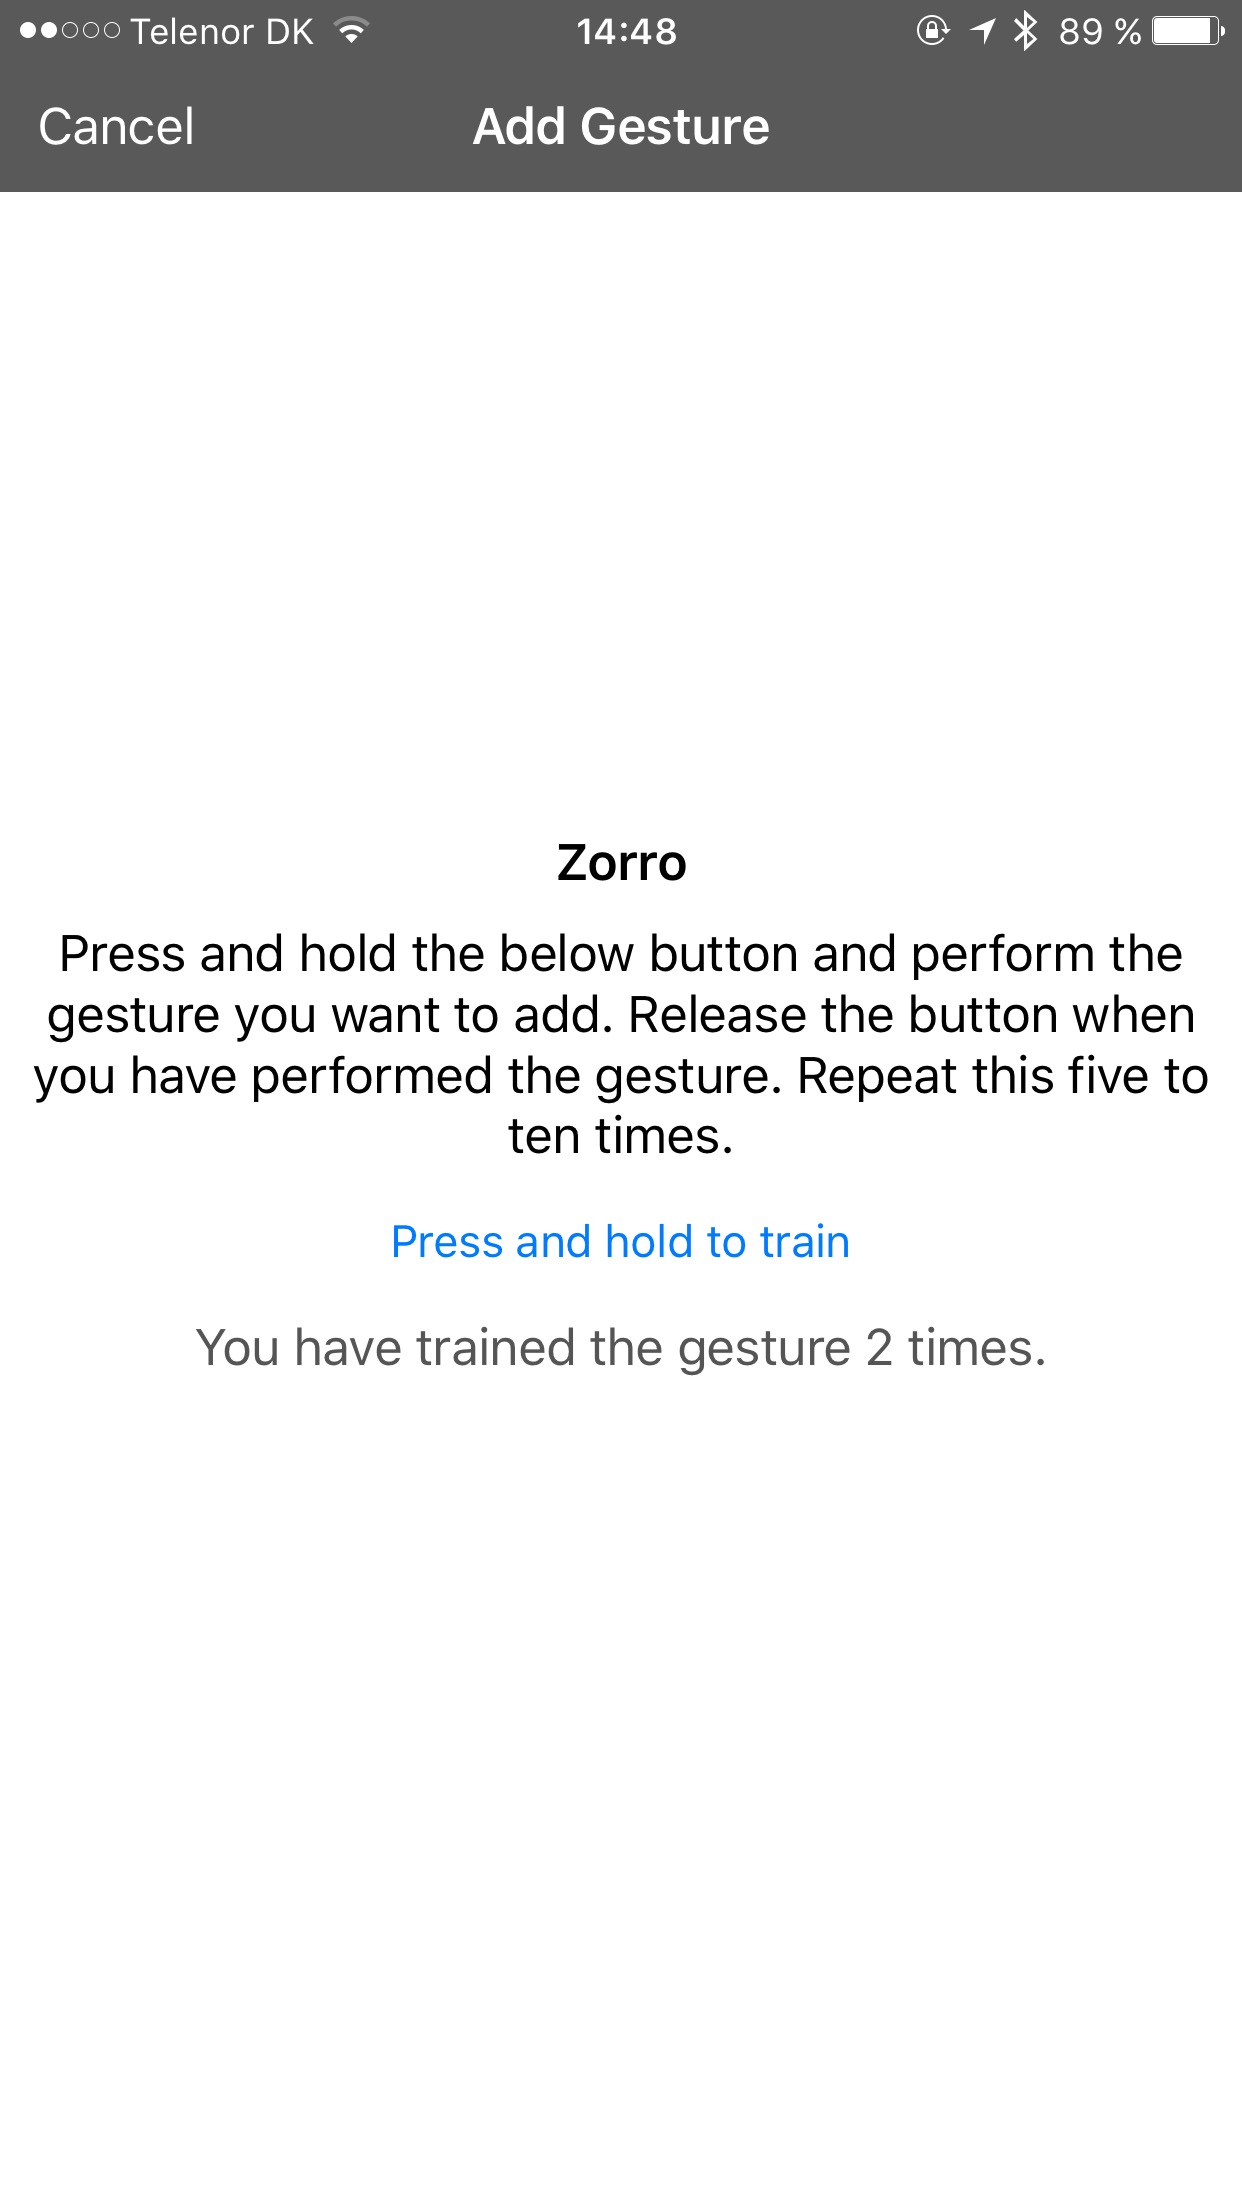
\includegraphics[width=0.3\textwidth]{images/prototype-3-train-gesture}
    }
    \caption{Screenshots showing the flow and interface for adding and training a new gesture in the third prototype.}
    \label{fig:prototype3-gesture-screenshots}
\end{figure}

\begin{figure}[!htb]%
    \centering
    \framebox{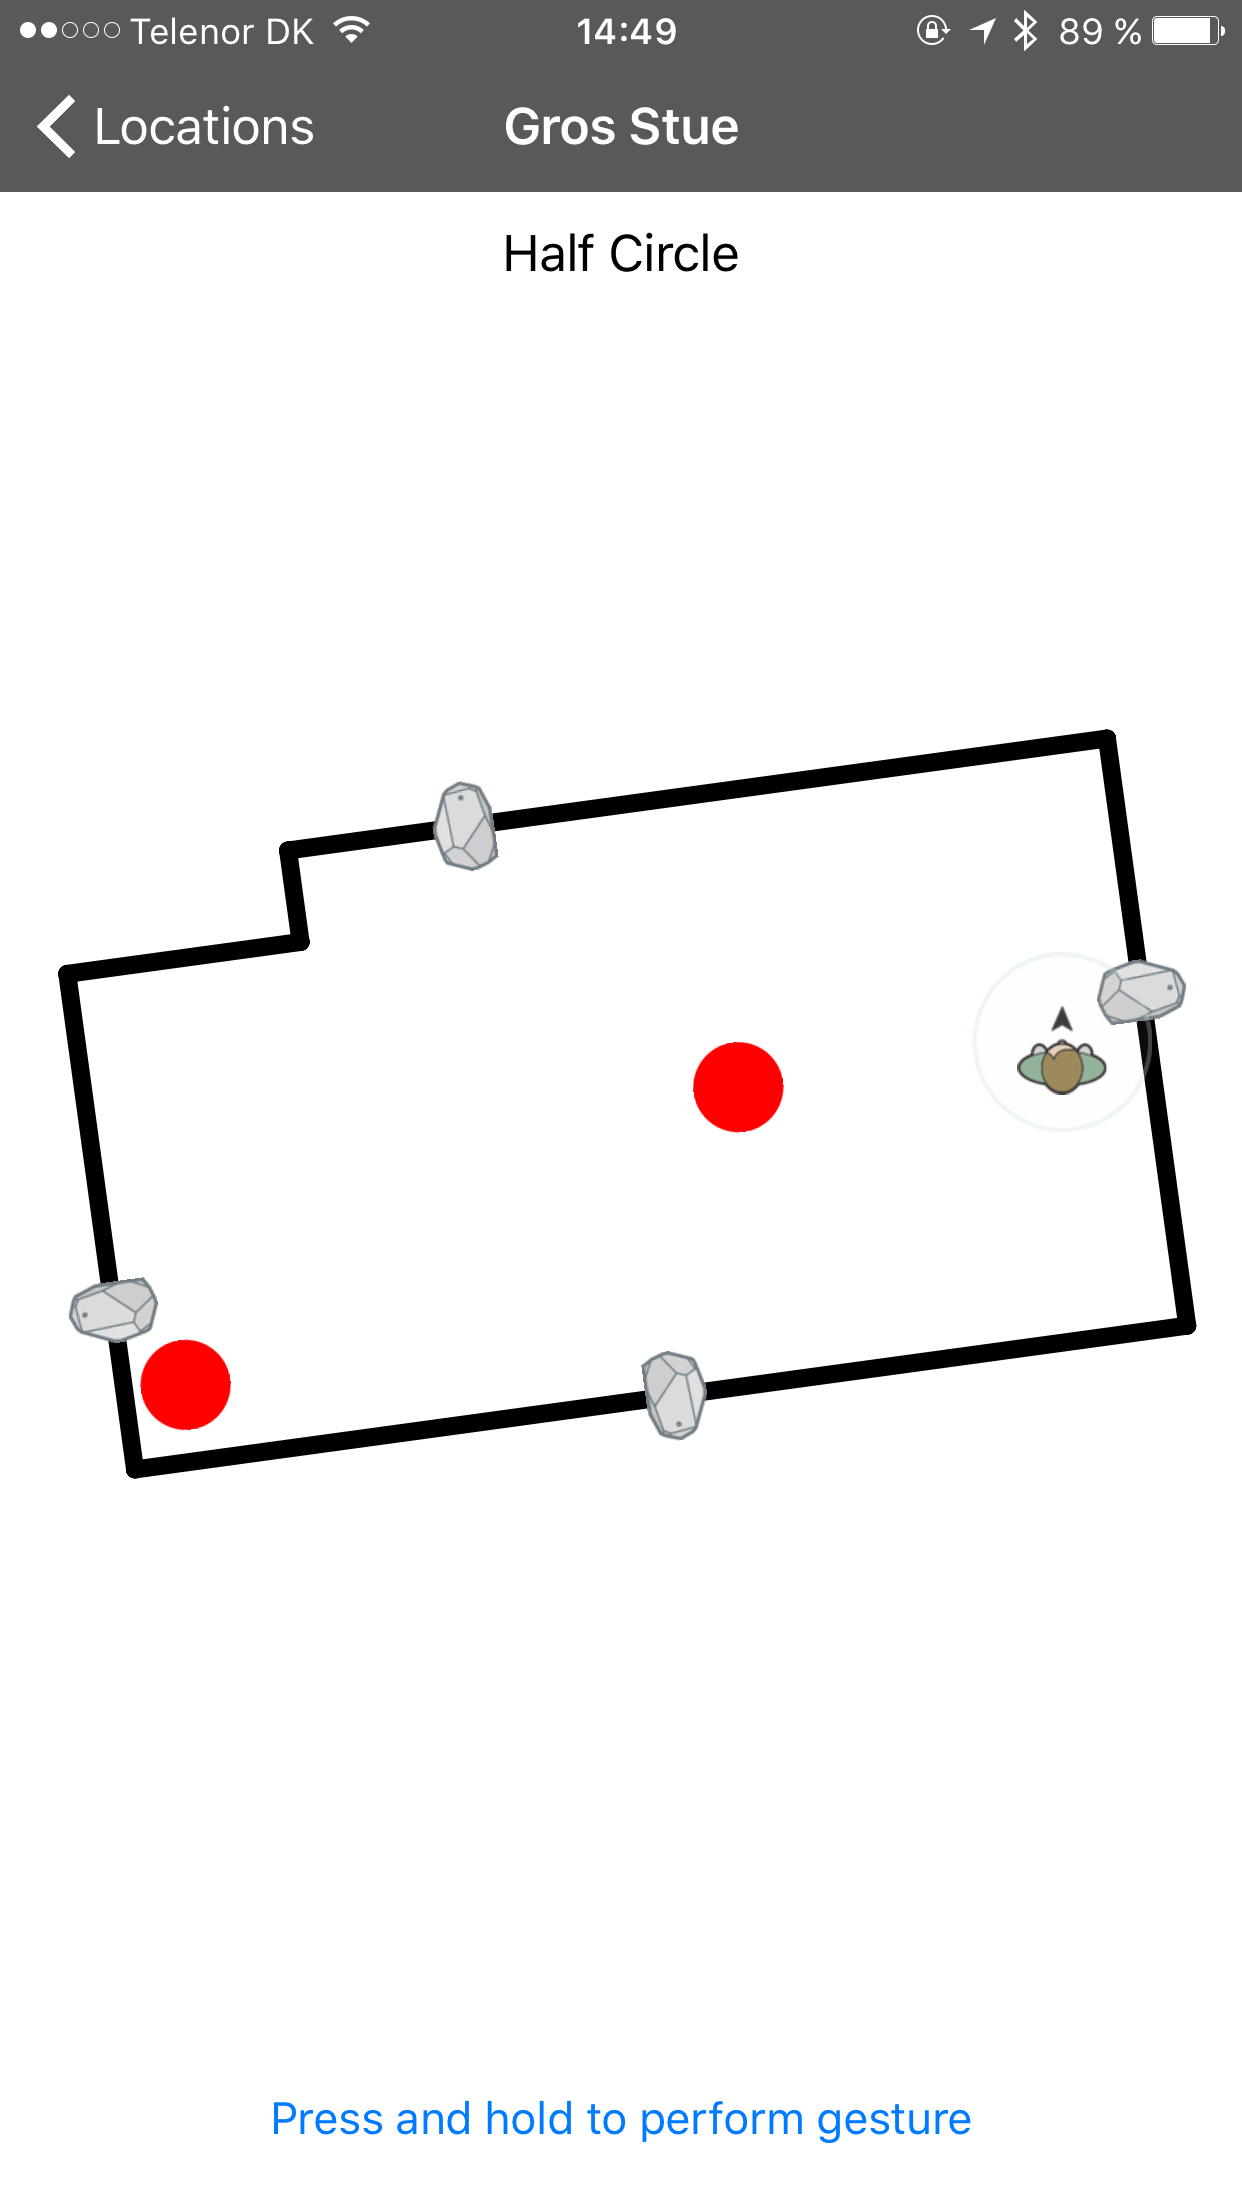
\includegraphics[width=0.3\textwidth]{images/prototype-3-gesture-triggered}}
    \caption{Screenshot showing new representation of the room and controllable devices. In this screenshot the gesture named ``Half Circle'' was recently recognized and therefore the gesture name is shown in the top of the screen.}
    \label{fig:prototype3-room-screenshot}
\end{figure}

%%% Local Variables:
%%% mode: latex
%%% TeX-master: "../../master"
%%% End:

This chapter describes the implementation details of our system, 
designed in \Cref{chap:design}. 
The system consists of three layers, as described by \Cref{fig:architecture}.
We designed the first layer to consist of a wearable device and a smartphone. 
However, since we did not have access to a wearable device, 
we have implemented the first layer entirely as a iPhone application. 

This application have been developed through several prototypes. 
The first prototype, described in \Cref{sec:implementation:prototypes:prototype1}, was implemented as an Android application, 
to develop a way to find which devices the user points at. 
\Cref{sec:implementation:prototypes:prototype2} describes the second prototype was implemented as a iPhone application,
developed to test communication with the server and control of the devices. 
We also developed a very basic server for this prototype, \ie the second layer. 
The third prototype in \Cref{sec:implementation:prototypes:prototype3}, 
implemented the \$3 Gesture Recognition system,
and used the location estimated from the Estimote SDK. 
The fourth and final prototype described in \Cref{sec:implementation:prototypes:prototype4} connected all the layers of the system. 
This prototype connects to and communicates with the implemented server and smart hub. 

The implementation of the server, \ie the second layer of the system, 
is described in \Cref{sec:serverimplementation}. 
As the smart hub, the third layer, is not something that we have implemented ourself, 
we will not describe the implementation of this.
However, \Cref{sec:serverimplementation} describes how it is connected to our system. 

\section{Prototype \#1}
\label{sec:implementation:prototypes:prototype1}
The purpose of the first prototype 
was to quickly test how to detect which devices users point at, 
given the user's position and the direction the user is facing, 
along with the underlying math.

\subsection{Description}
The first prototype was an Android phone application, 
that showed the devices that the user pointed at.
The application used a $10 \times 10$ grid to simulate a square room, 
in which the user and the devices to be controlled were located.
A set of imaginary devices was hardcoded into the application with fixed positions, 
and the grid would look like the one shown in \Cref{table/prototype-grid}.
The user is positioned in the center at $(5,5)$ by default. 
This position can be changed by using the \texttt{Up}, \texttt{Down}, \texttt{Left} and \texttt{Right} buttons.
When the user's direction changes, 
a list of devices being pointed at is acquired, 
by calculating the angle between the user's position and the position of each device.
The direction is found using magnetic fields\todo[author=Brian]{Kan højtalere og andre magnetiske felter forstyrre magnetometeret så det ikke længere er præcist nok?}, 
such that \num{0} is north, \num{-90} is west, \num{90} is east, etc. 

The angle between each smart device and the user, 
is calculated by \Cref{eq:angle} from \Cref{sec:analysis:orientation}:
\begin{equation}
\var{angle} = 180 / \pi * \arctan(\var{user.y} - \var{device.y} / \var{user.x} - \var{device.x})
\end{equation}
where \var{user.x} and \var{user.y} are the $x$ and $y$ coordinates of the user and likewise for the device.
A screenshot of this application is shown in \Cref{fig:prototype1-app-screenshots}.

% Thalley: Måske lave om et et Tikz coordinatsystem i stedet for? Fylder unødvendigt meget imo. 
\begin{table}[!htb] 
    \centering
    \tiny
    \begin{TAB}(e){|c:c:c:c:c:c:c:c:c:c|}{|c:c:c:c:c:c:c:c:c:c|}
     &  &  &  &  &  &  &  &  & Stereo \\
     &  &  &  &  &  &  &  &  &  \\
     &  &  &  &  &  & \begin{tabular}[c]{@{}l@{}}Coffee\\ Maker\end{tabular} &  &  &  \\ 
     &  &  &  &  &  &  &  &  &  \\ 
    \begin{tabular}[c]{@{}l@{}}Garage\\ Door\end{tabular} &  &  &  &  &  &  &  &  &  \\ 
     &  & Lamp 2 &  &  &  &  &  &  &  \\
     &  &  &  &  &  &  &  &  &  \\ 
     &  &  &  &  &  &  &  &  &  \\ 
     &  &  &  &  &  &  &  &  &  \\ 
    Lamp 1 &  &  &  &  & TV &  &  &  &  \\
    \end{TAB}    
    \caption{A $10 \times 10$ grid showing the position of devices. Lamp 1 is located at $(0,0)$ and Stereo is located at $(9,9)$}
    \label{table/prototype-grid}
\end{table}

\subsection{Results}

From the prototype we found that given the user's position, 
the user's orientation provided by a magnetometer and the positions of smart devices, 
we can determine which smart devices a user points at. 
We were also able to determine the math needed to check which smart devices the user points at.

Based on this we can expand the prototype, 
to work with dynamically loaded devices, 
and perform actions on the smart devices being pointed at.

\begin{figure}[!htb]%
    \centering
    \subfloat{
        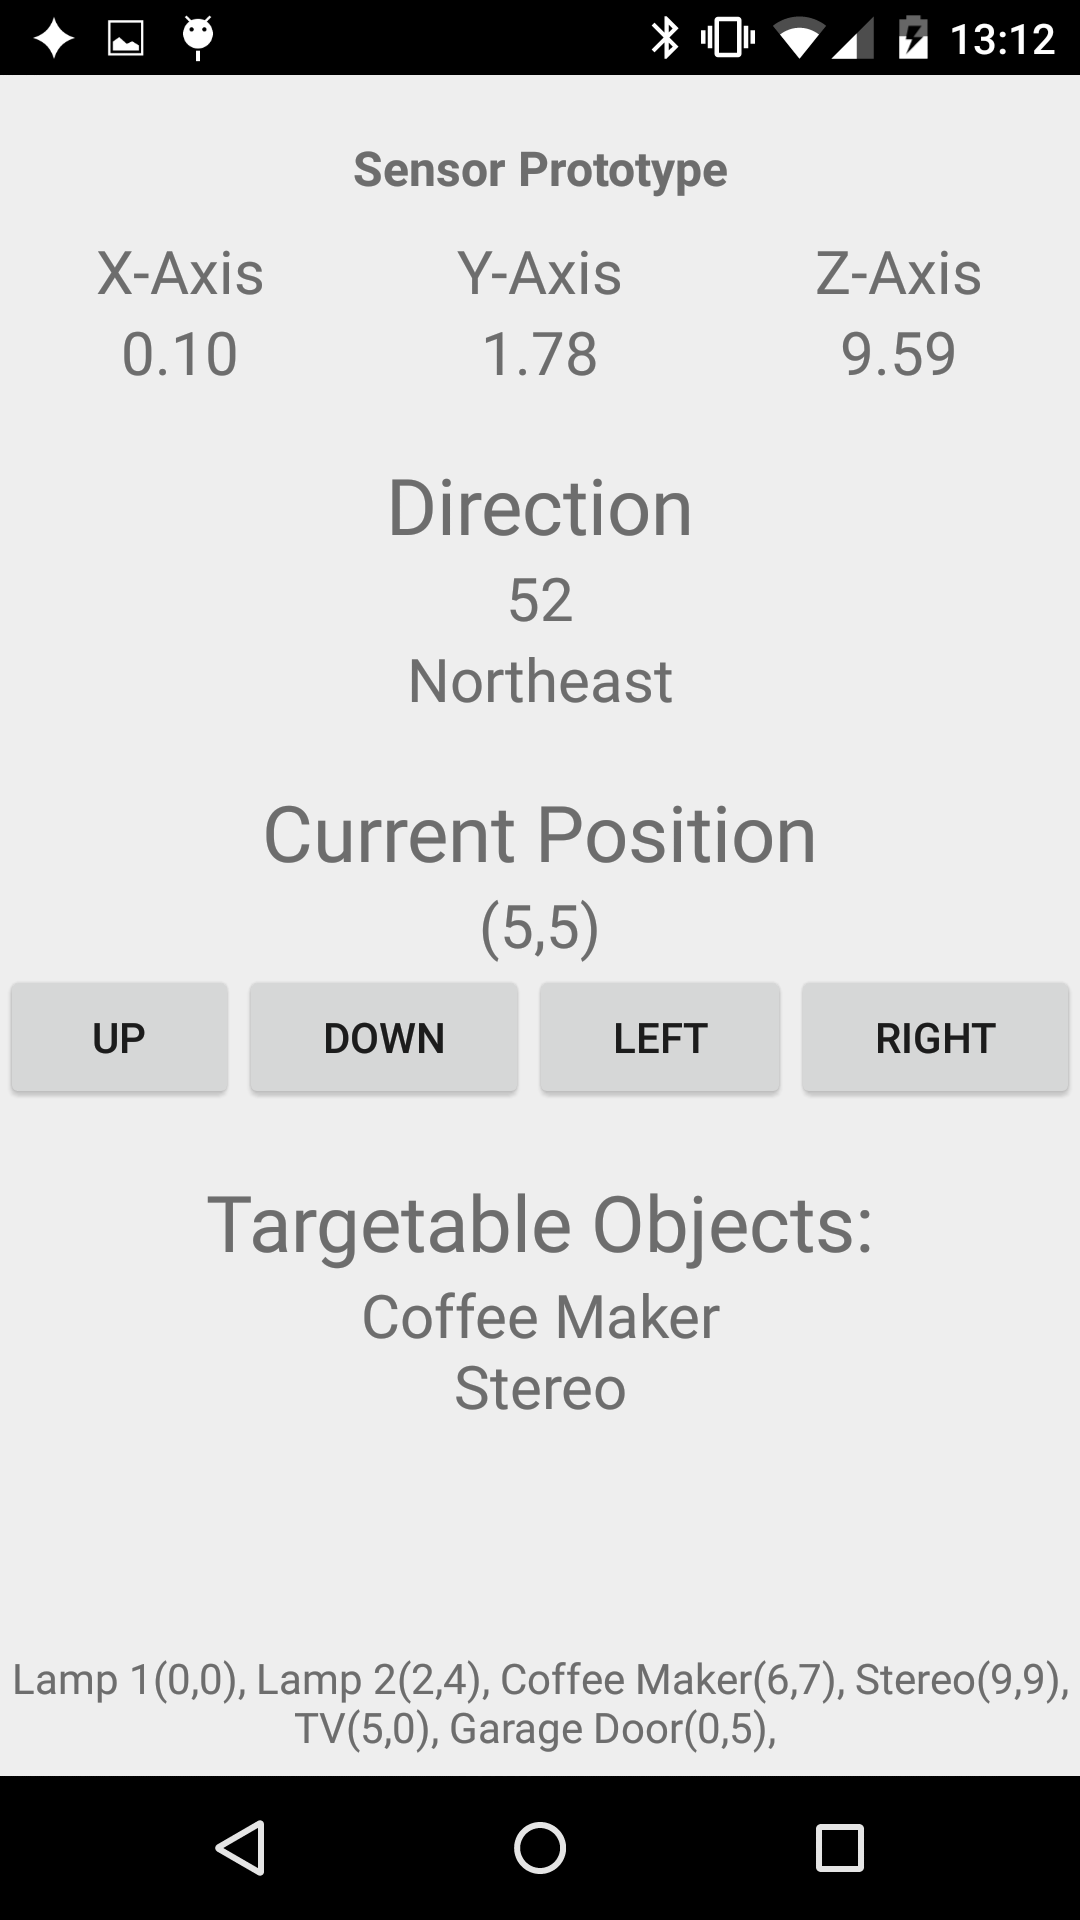
\includegraphics[width=0.3\textwidth]{images/Prototype1_Android_1.png}
    }
    \subfloat{
        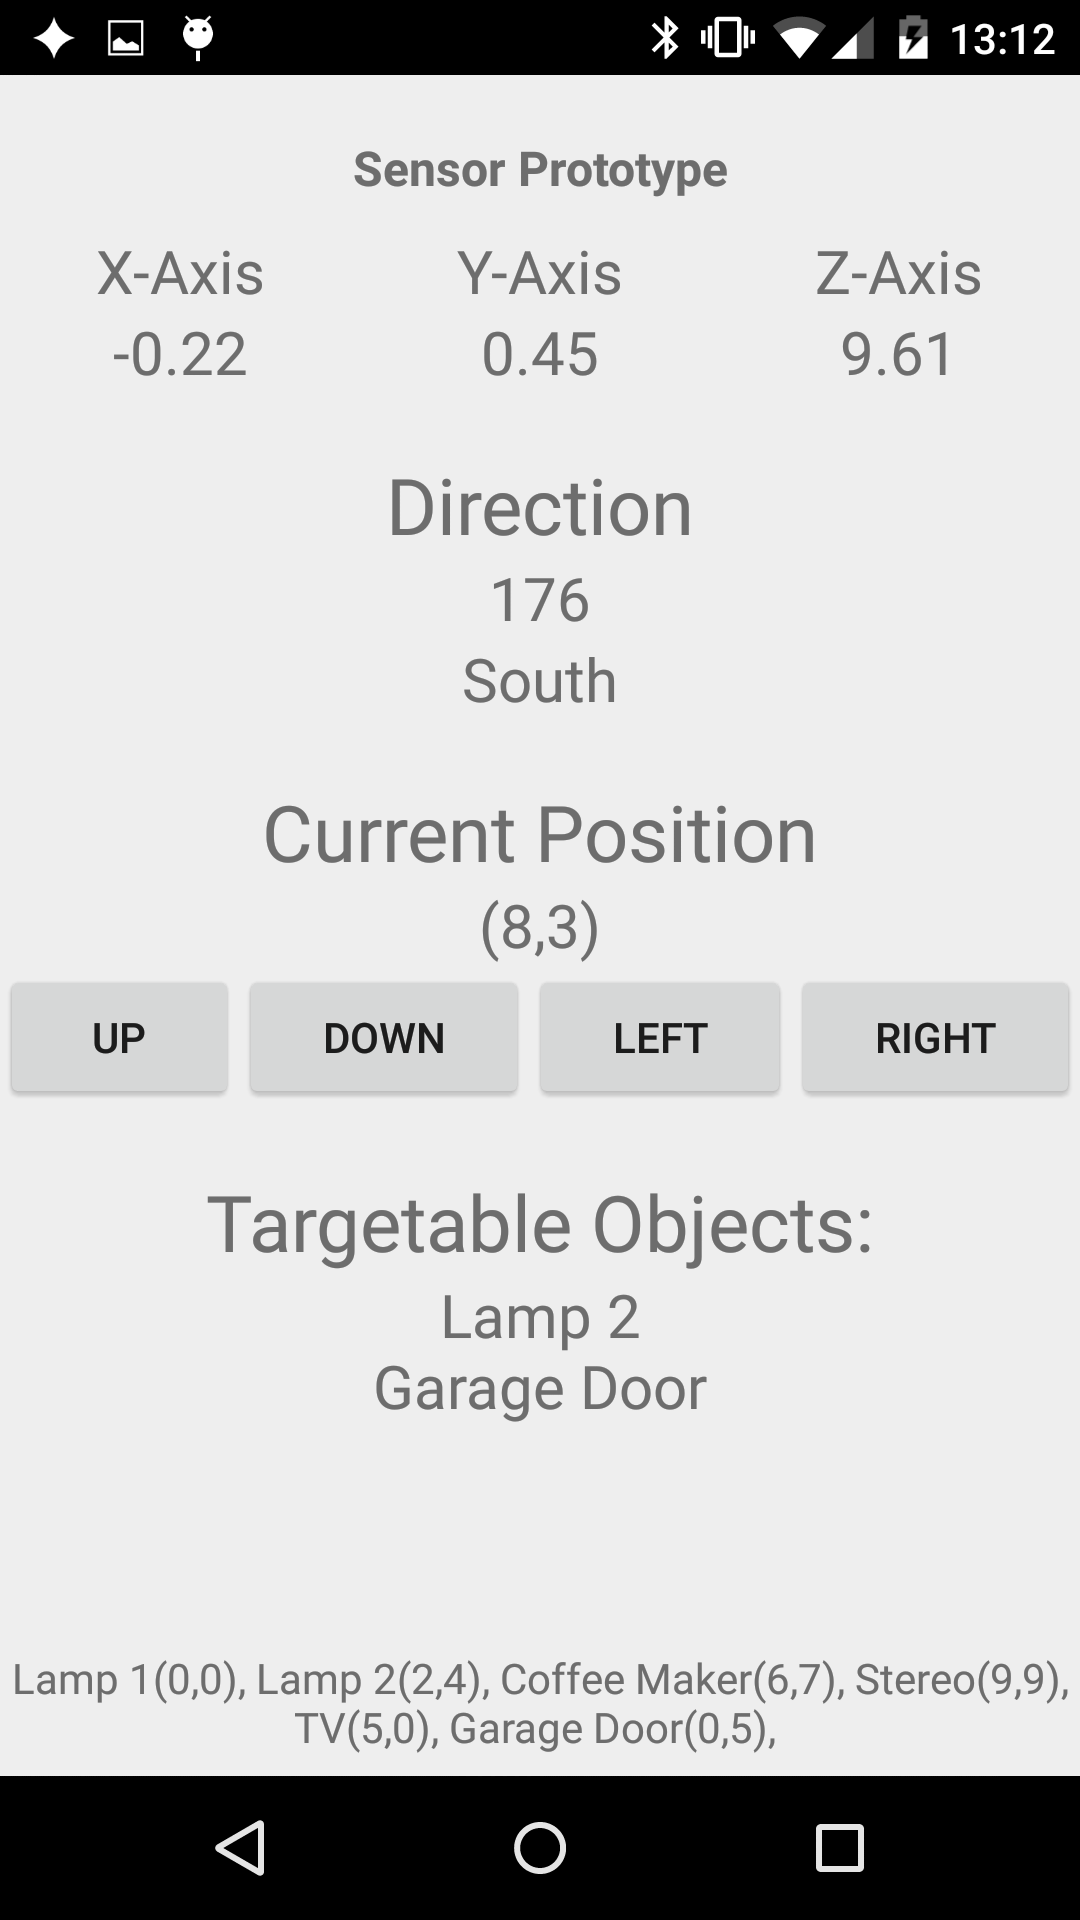
\includegraphics[width=0.3\textwidth]{images/Prototype1_Android_2.png}
    }
    \caption{Screenshots of the first prototype.}
    \label{fig:prototype1-app-screenshots}
\end{figure}

%%% Local Variables:
%%% mode: latex
%%% TeX-master: "../../master"
%%% End:

\FloatBarrier
\subsection{Prototype \#2}
\label{sec:implementation:prototypes:prototype2}
\subsubsection{Purpose}
The purpose of the second prototype, 
was to test the indoor positioning of the user, 
using Estimote beacons, 
and determine if gesture recognition can be performed, 
using the hardware of a smartphone.

\subsubsection{Description}
The second prototype consisted of an iOS application, 
similar to the Android application described in \Cref{sec:implementation:prototypes:prototype1}, 
and a server that represented two controllable lamps.
The platform was changed from Android to iOS, 
because Estimote does not have a SDK for Android.

In this prototype the room was still represented as a grid, 
and the user was placed in the center of the grid, 
however the user was unable to change position.
This is because the first prototype showcased the idea of pointing at devices from different locations sufficiently, 
and the next step would be to use the actual location of a user using Estimote beacons.
As shown in \Cref{fig:prototype2-app-screenshots}, 
the user can see his direction as an angle between himself and north.
The angle is computed the same way as in Prototype 1 with \Cref{eq:angle}.

Devices are represented as orange dots, 
and if the user points towards one of them, 
two buttons will appear that allow the user to interact with the device, 
by either turning it \texttt{on} or \texttt{off}.
When the user turns a device on or off, 
it will be reflected on the server, 
where a corresponding box will have the color \texttt{green} when turned on, 
and \texttt{red} when turned off as shown in \Cref{fig:prototype2-server-screenshot}.
The server is running as a Heruko\footnote{\url{https://heroku.com/}} application, 
as a simple RESTful webservice written in Python. 
The server contains the information of the devices, 
such as ID, name, status and position.
The application gets this information by sending a GET request, 
to get a list of all the devices and their information. 
To change the status of a device (turn off or on), 
the application sends a POST request with the device's ID and the action. 
In this prototype, the only actions are \texttt{turnOn} and \texttt{turnOff}.

\subsubsection{Major Changes}
\begin{itemize}
    \item Introduction of a server for the application to interact with.
    \item Switched platform from Android to iOS.
\end{itemize}

\subsubsection{Results}

We were able to point at one or more devices,
and send an action to the devices, 
in order to flip between their two different states. 
Both the user's position and the devices were simulated.

The next step is to perform actual indoor positioning of the user.

\begin{figure}[!htb]%
    \centering
    \subfloat{
        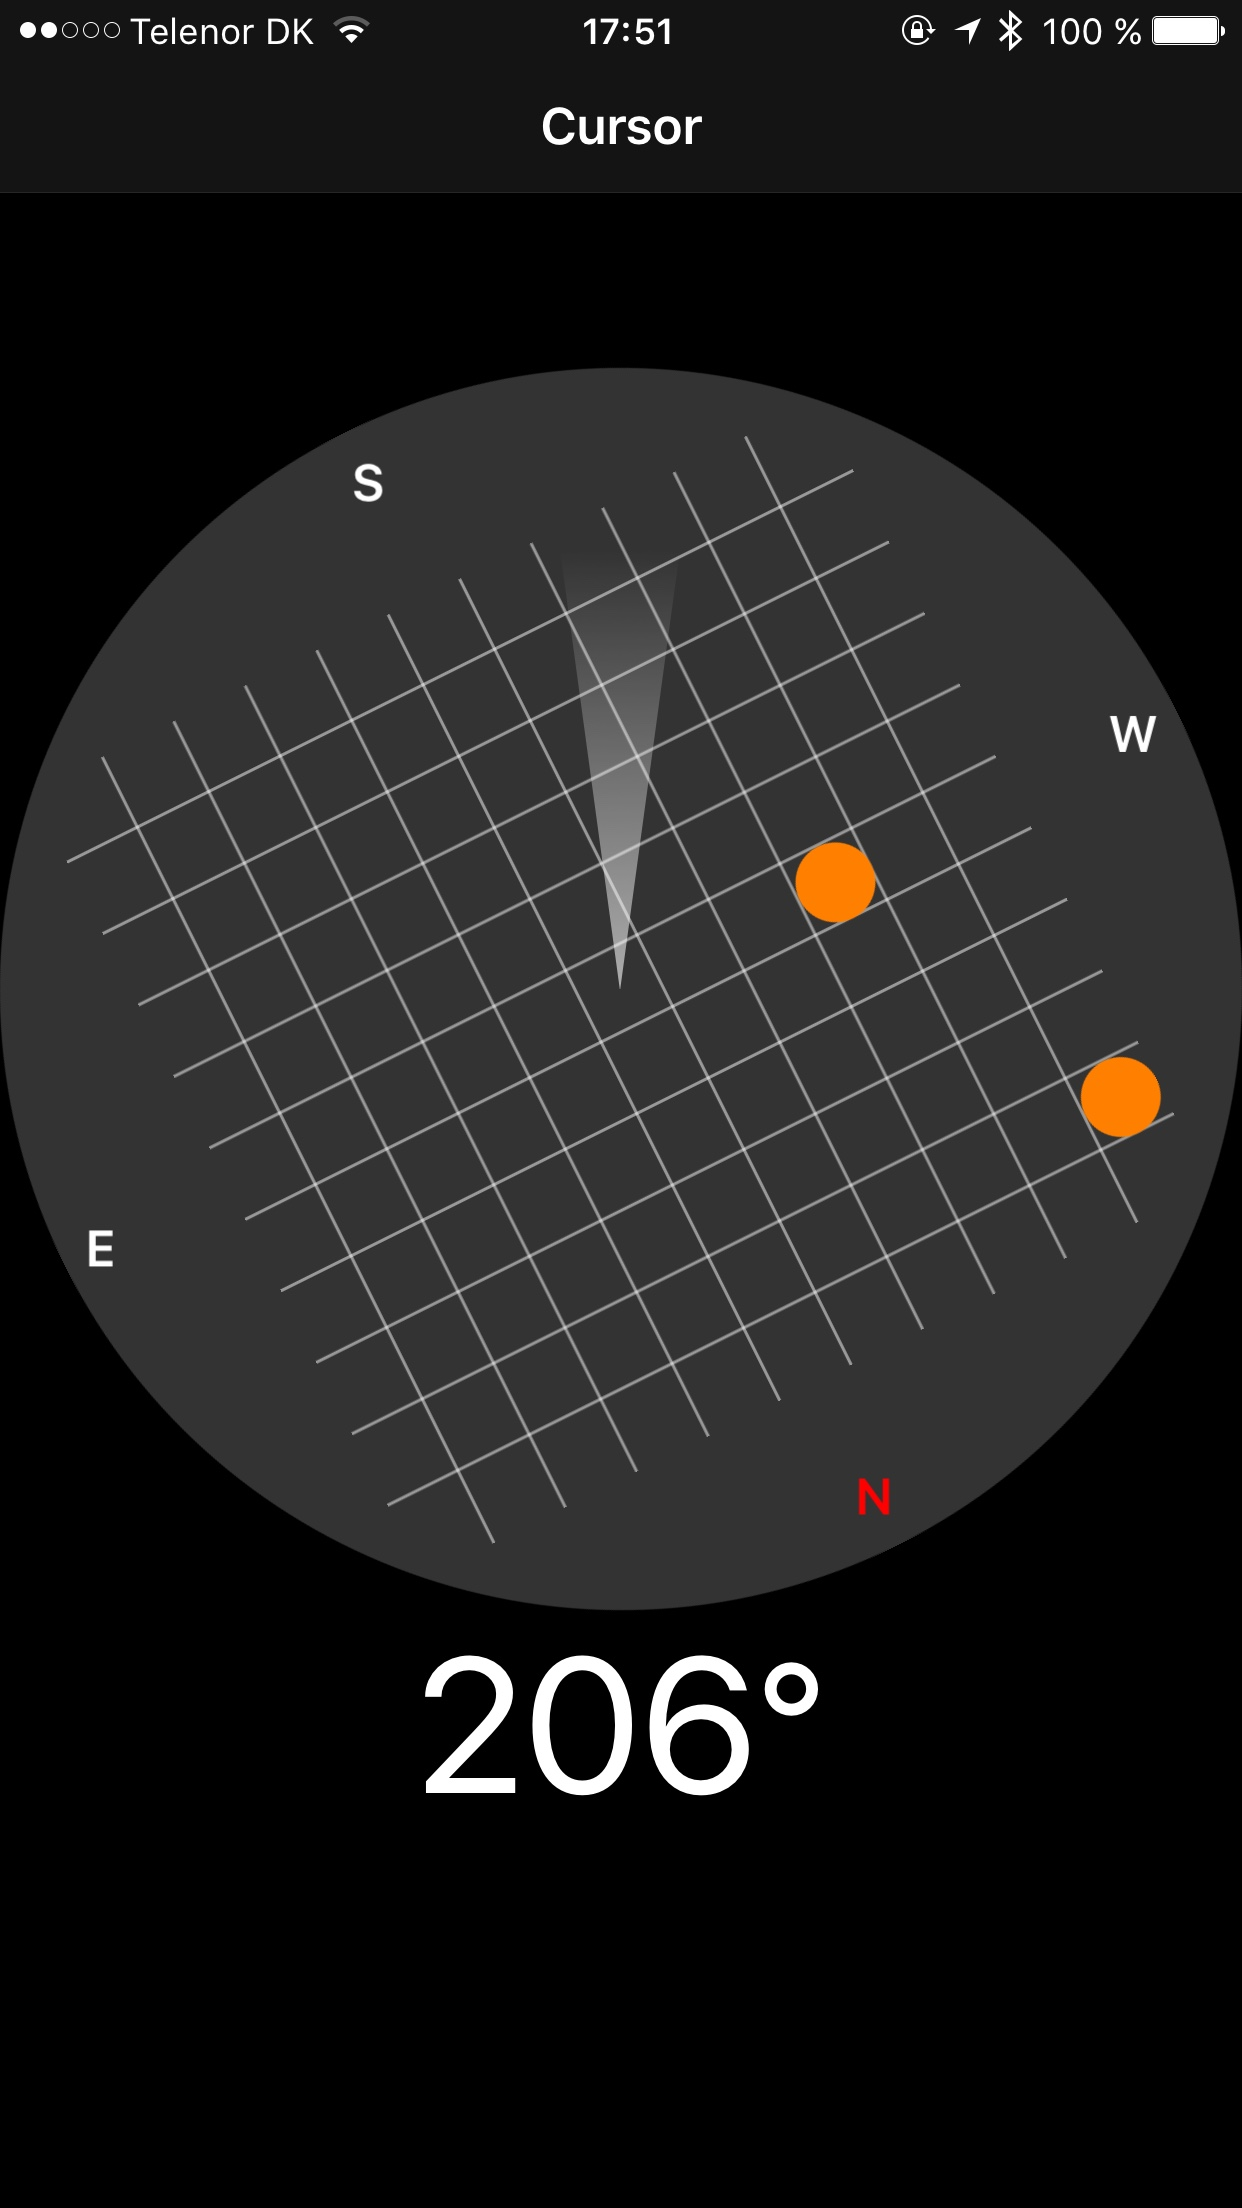
\includegraphics[width=0.3\textwidth]{images/Prototype2_iOS_1.png}
    }
    \subfloat{
        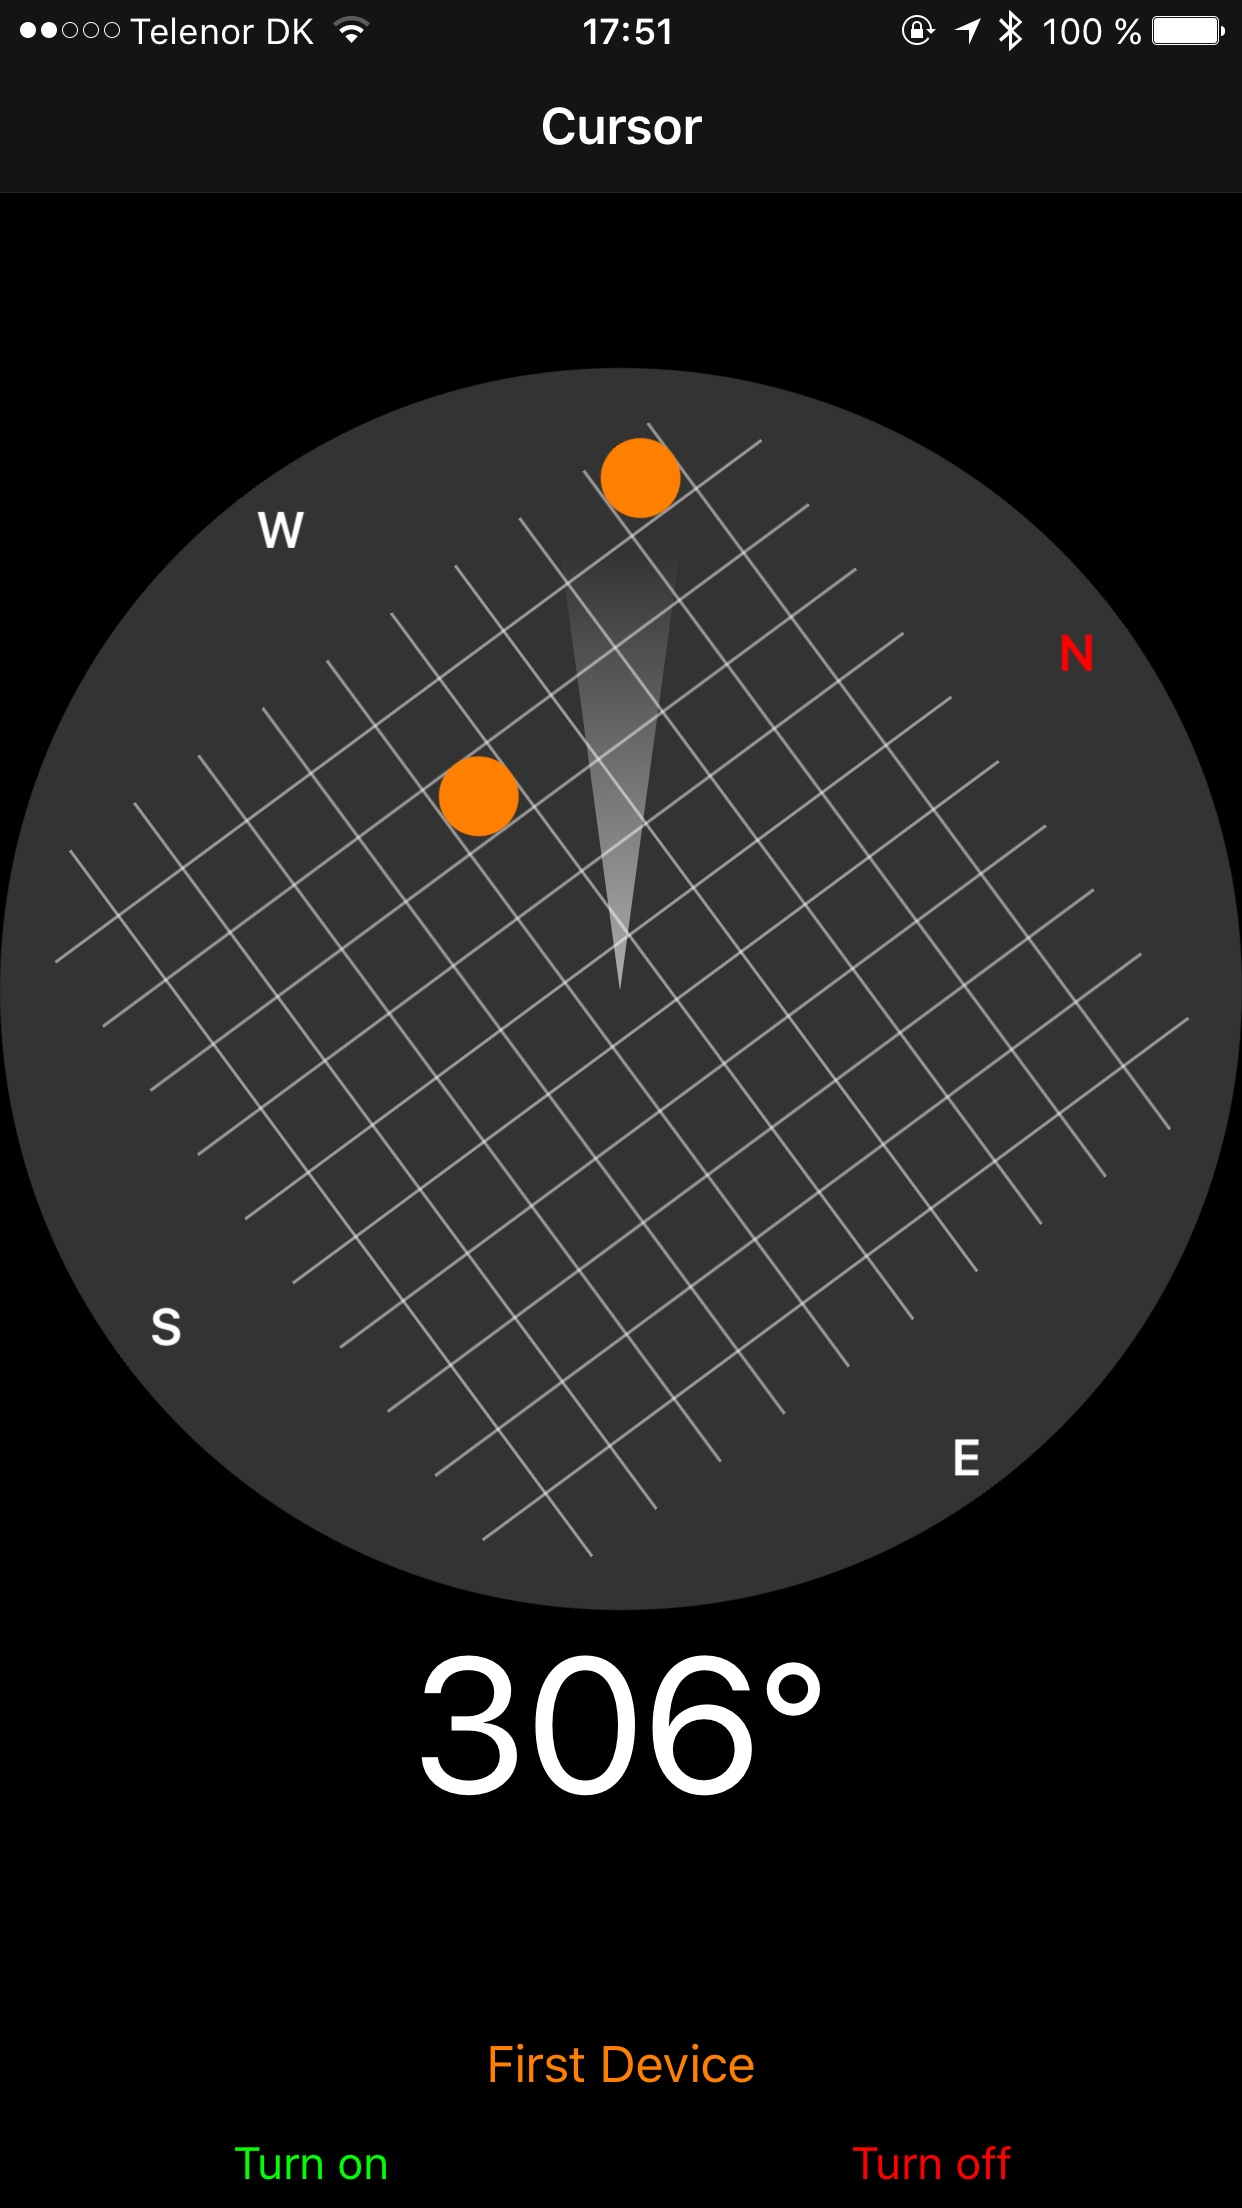
\includegraphics[width=0.3\textwidth]{images/Prototype2_iOS_2.png}
    }
    \caption{Screenshots of the second prototype application.}
    \label{fig:prototype2-app-screenshots}
\end{figure}

\begin{figure}[!htb]
    \centering
    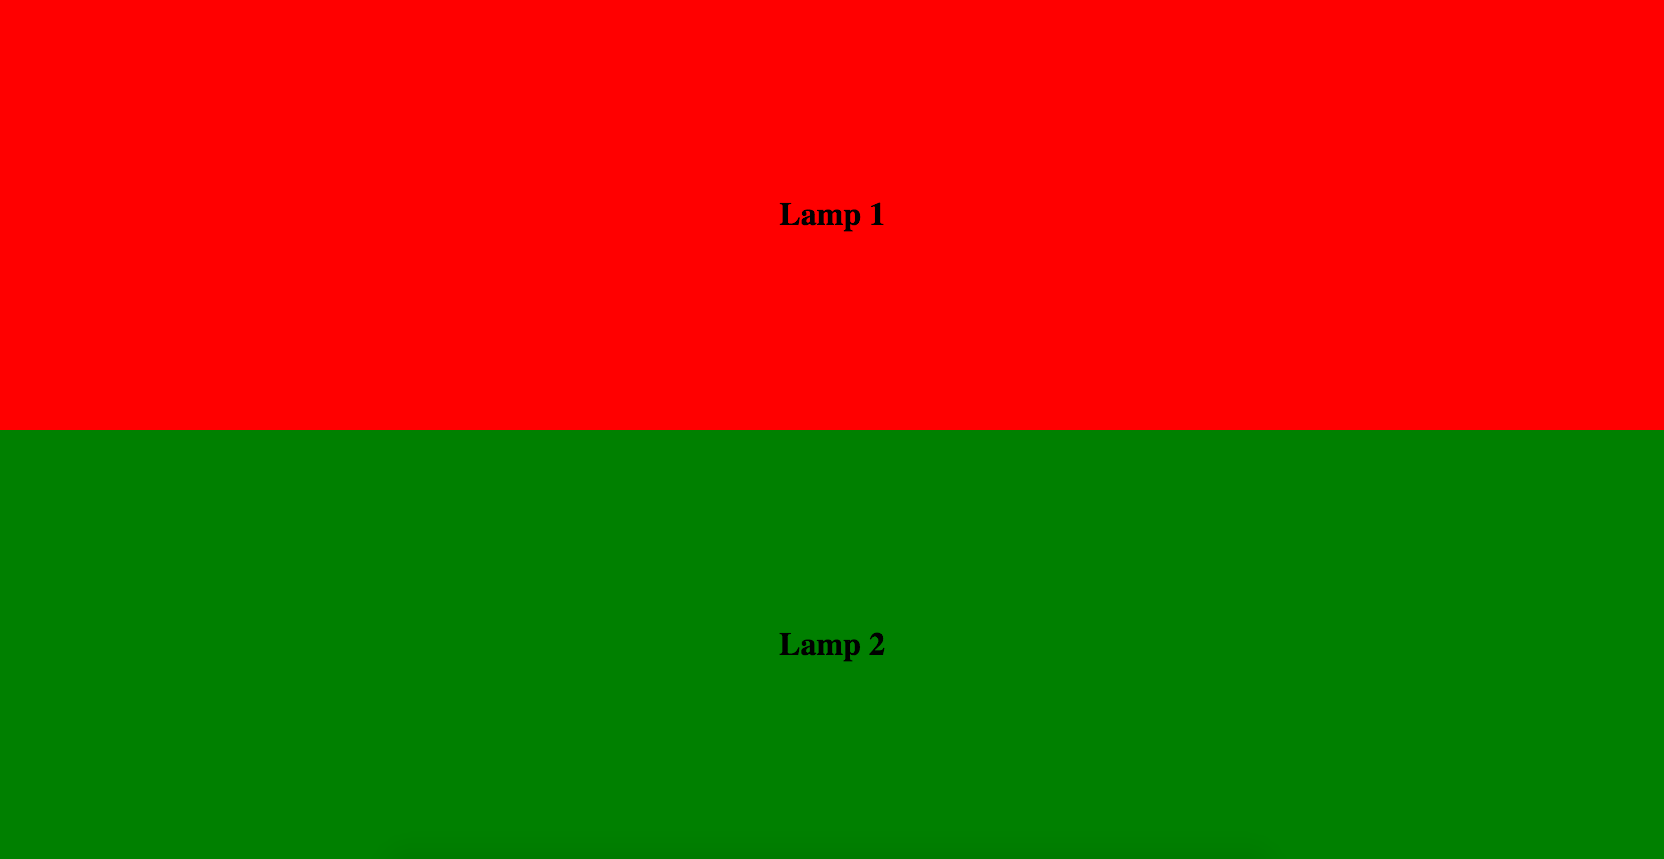
\includegraphics[width=0.8\textwidth]{images/Prototype2_Server.png}
    \caption{Screenshot of the server representing two lamps in the second prototype. Colors indicate their status. \texttt{Red} (top): Off and \texttt{Green} (bottom): On}
    \label{fig:prototype2-server-screenshot}
\end{figure}

%%% Local Variables:
%%% mode: latex
%%% TeX-master: "../../master"
%%% End:

\FloatBarrier
\section{Prototype \#3}
\label{sec:implementation:prototypes:prototype3}

The purpose of the third prototype, 
was to test indoor positioning using the Estimote beacons, 
as well as test the use of gesture recognition on a smartphone.

\subsection{Description}
The third prototype builds upon the second prototype for iOS, 
which was expanded to include some new features. 
The second prototype would assume that the user was positioned in the center of the room, 
but the new prototype takes the users position into account when determining devices being pointed at. 
Estimote beacons and the SDK provided by Estimote for indoor positioning was utilized, 
in order to determine the position of the user.

The indoor SDK from Estimote provides a visualization of the room, 
in which the positioning takes place, 
as well as a visualization of the installed beacons, 
and the position of the user. 
The view can be used to visualize custom objects. 
\Cref{fig:prototype3-room-screenshot} shows two red circles in the room. 
Each of the circles represent one of the virtual lamps introduced in the second prototype. 
The color of the lamp indicates the state the lamp is in. 
A lamp can either be on or off. 
The states are represented by green and red respectively.

Furthermore the prototype added support for training and recognizing gestures, 
using the \threedollar library described in \Cref{sec:threedollar}.
Users can add a gesture by giving the gesture a name, 
and train it at least \num{5} times. 
When added, the gesture can be used when pointing at a lamp, 
to toggle the state of the lamp. 
For example, if the user has trained a circle named ``Half Circle'', 
he can visit the screen showing his lamps and his position, 
point at one or more lamps and perform the ``Half Circle'' gesture, 
in order to either turn on or turn off the lamps.

The third prototype does not support associating a gesture with an action, 
\ie performing a specific action for a specific gesture. 
Nor does it support creating a model of a room. 
The prototype is limited to a specific (hardcoded) room,
modeled after the living room of one of the research members.

\subsection{Major Changes}
\begin{itemize}
\item Uses BLE beacons to position the user in a room, and take his position into account, when determining devices being pointed at.
\item Adds training and recognition of gestures, in order to trigger actions of a controllable device.
\item Adds a graphical representation of the room, in which the beacons and the devices are installed.
\end{itemize}

\subsection{Results}

We were able to get the position of the user by using Estimote beacons, 
allowing the application to keep track of the user. 
In addition, the \threedollar library was introduced, 
which allows users to control the lamps by performing a gesture with the phone.
The accuracy of Estimote is explored in \Cref{sec:estimoteprecision}, 
and the performance of the gesture recognition is explored in \Cref{sec:gestureperformance}.

The prototype used simulated devices, 
and the next step is to control actual smart devices, 
and give the user a more fine grained control, 
over which devices are controlled when performing a gesture.

\begin{figure}[!htb]%
    \centering
    \subfloat{
        \frame{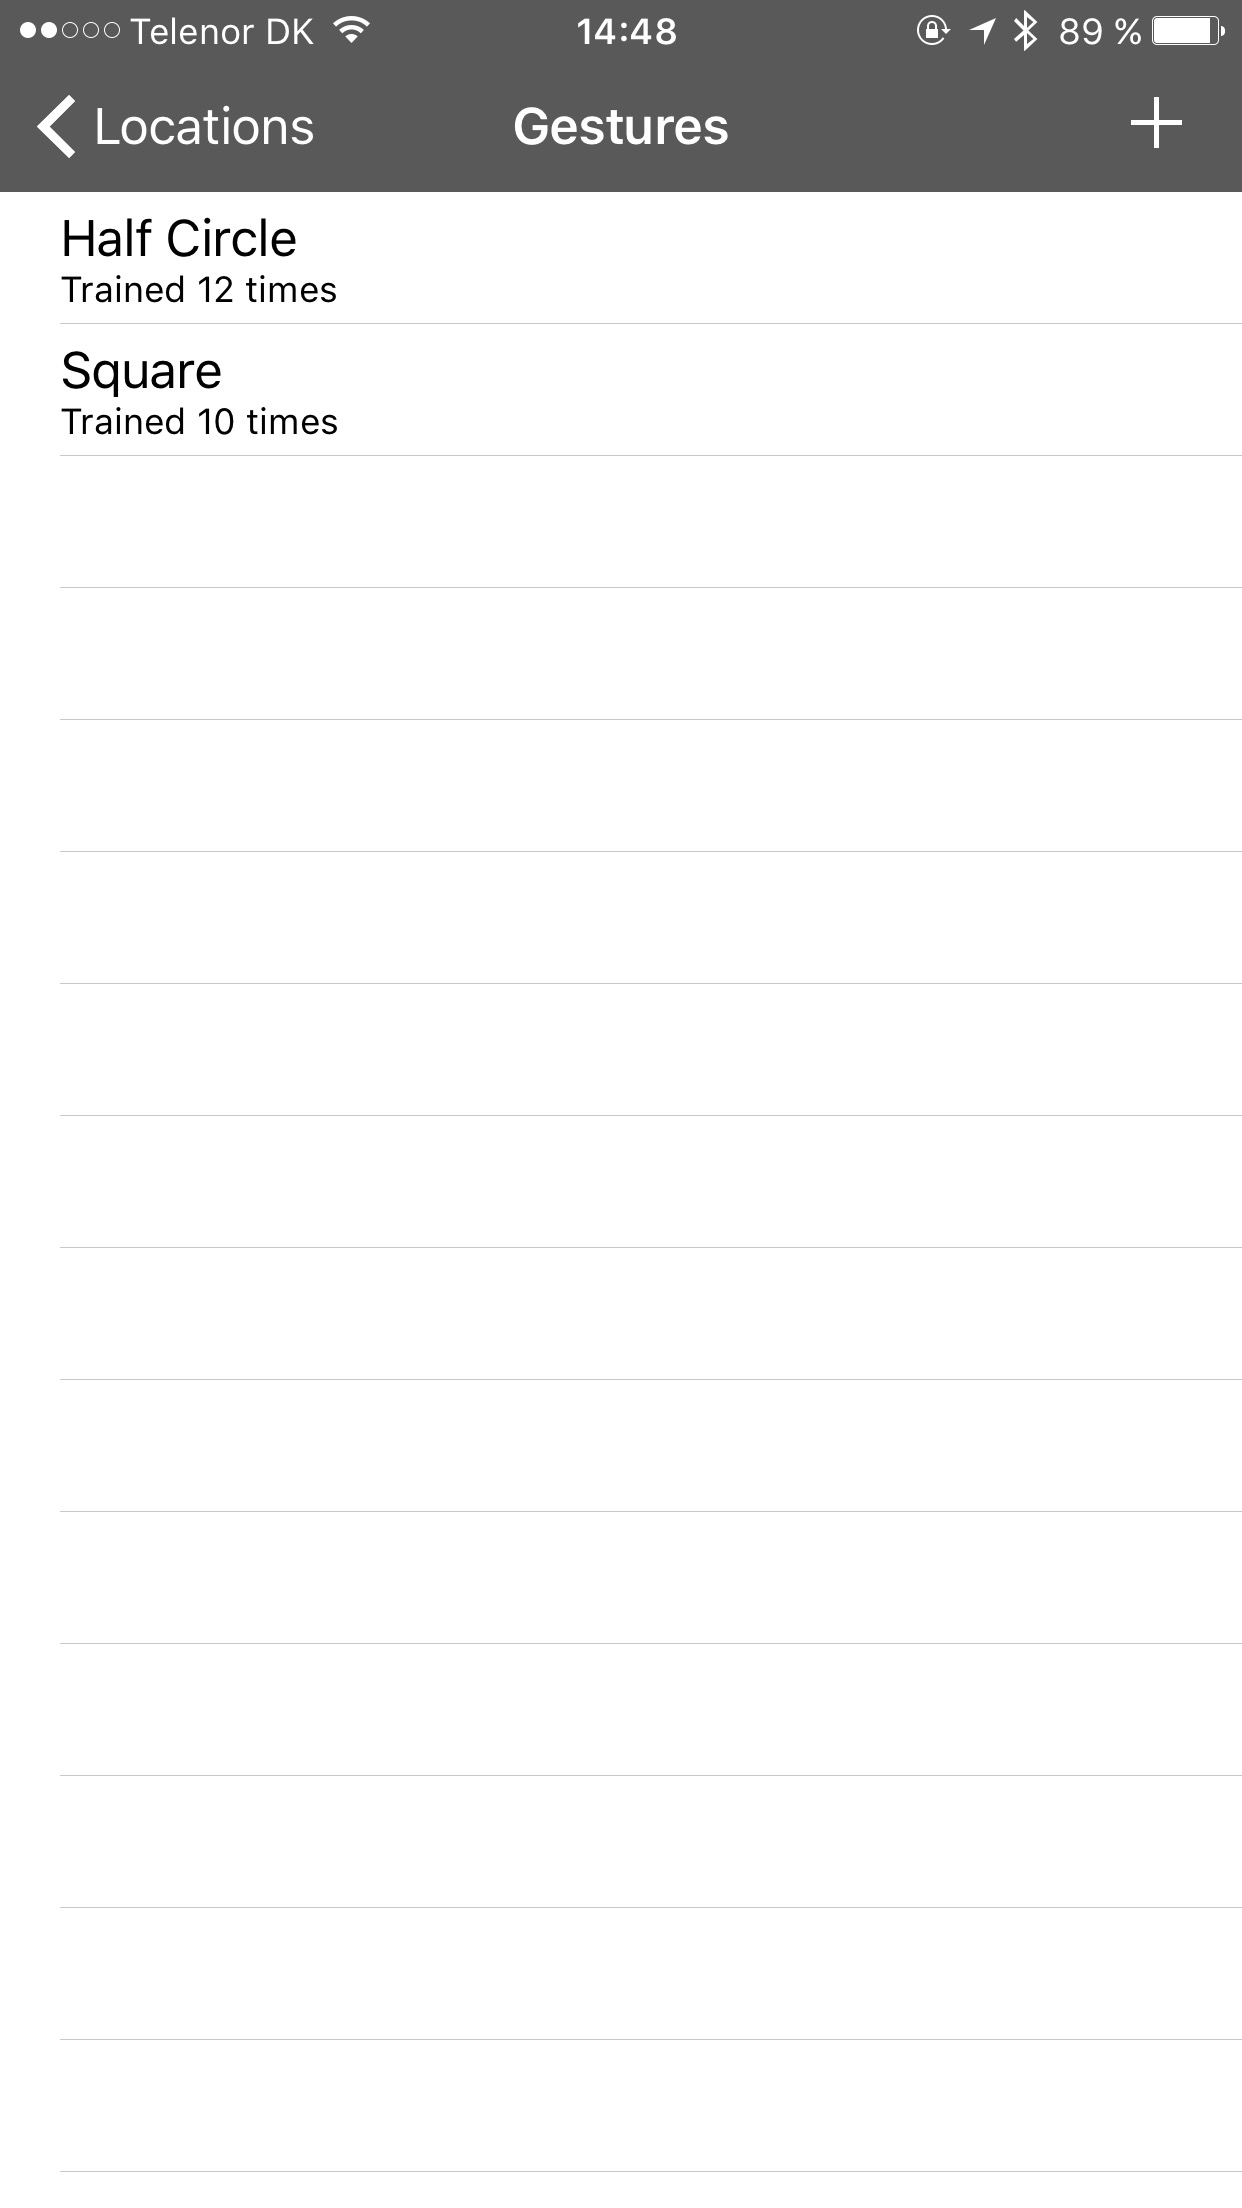
\includegraphics[width=0.3\textwidth]{images/prototype-3-all-gestures}}
    }
    \subfloat{
        \frame{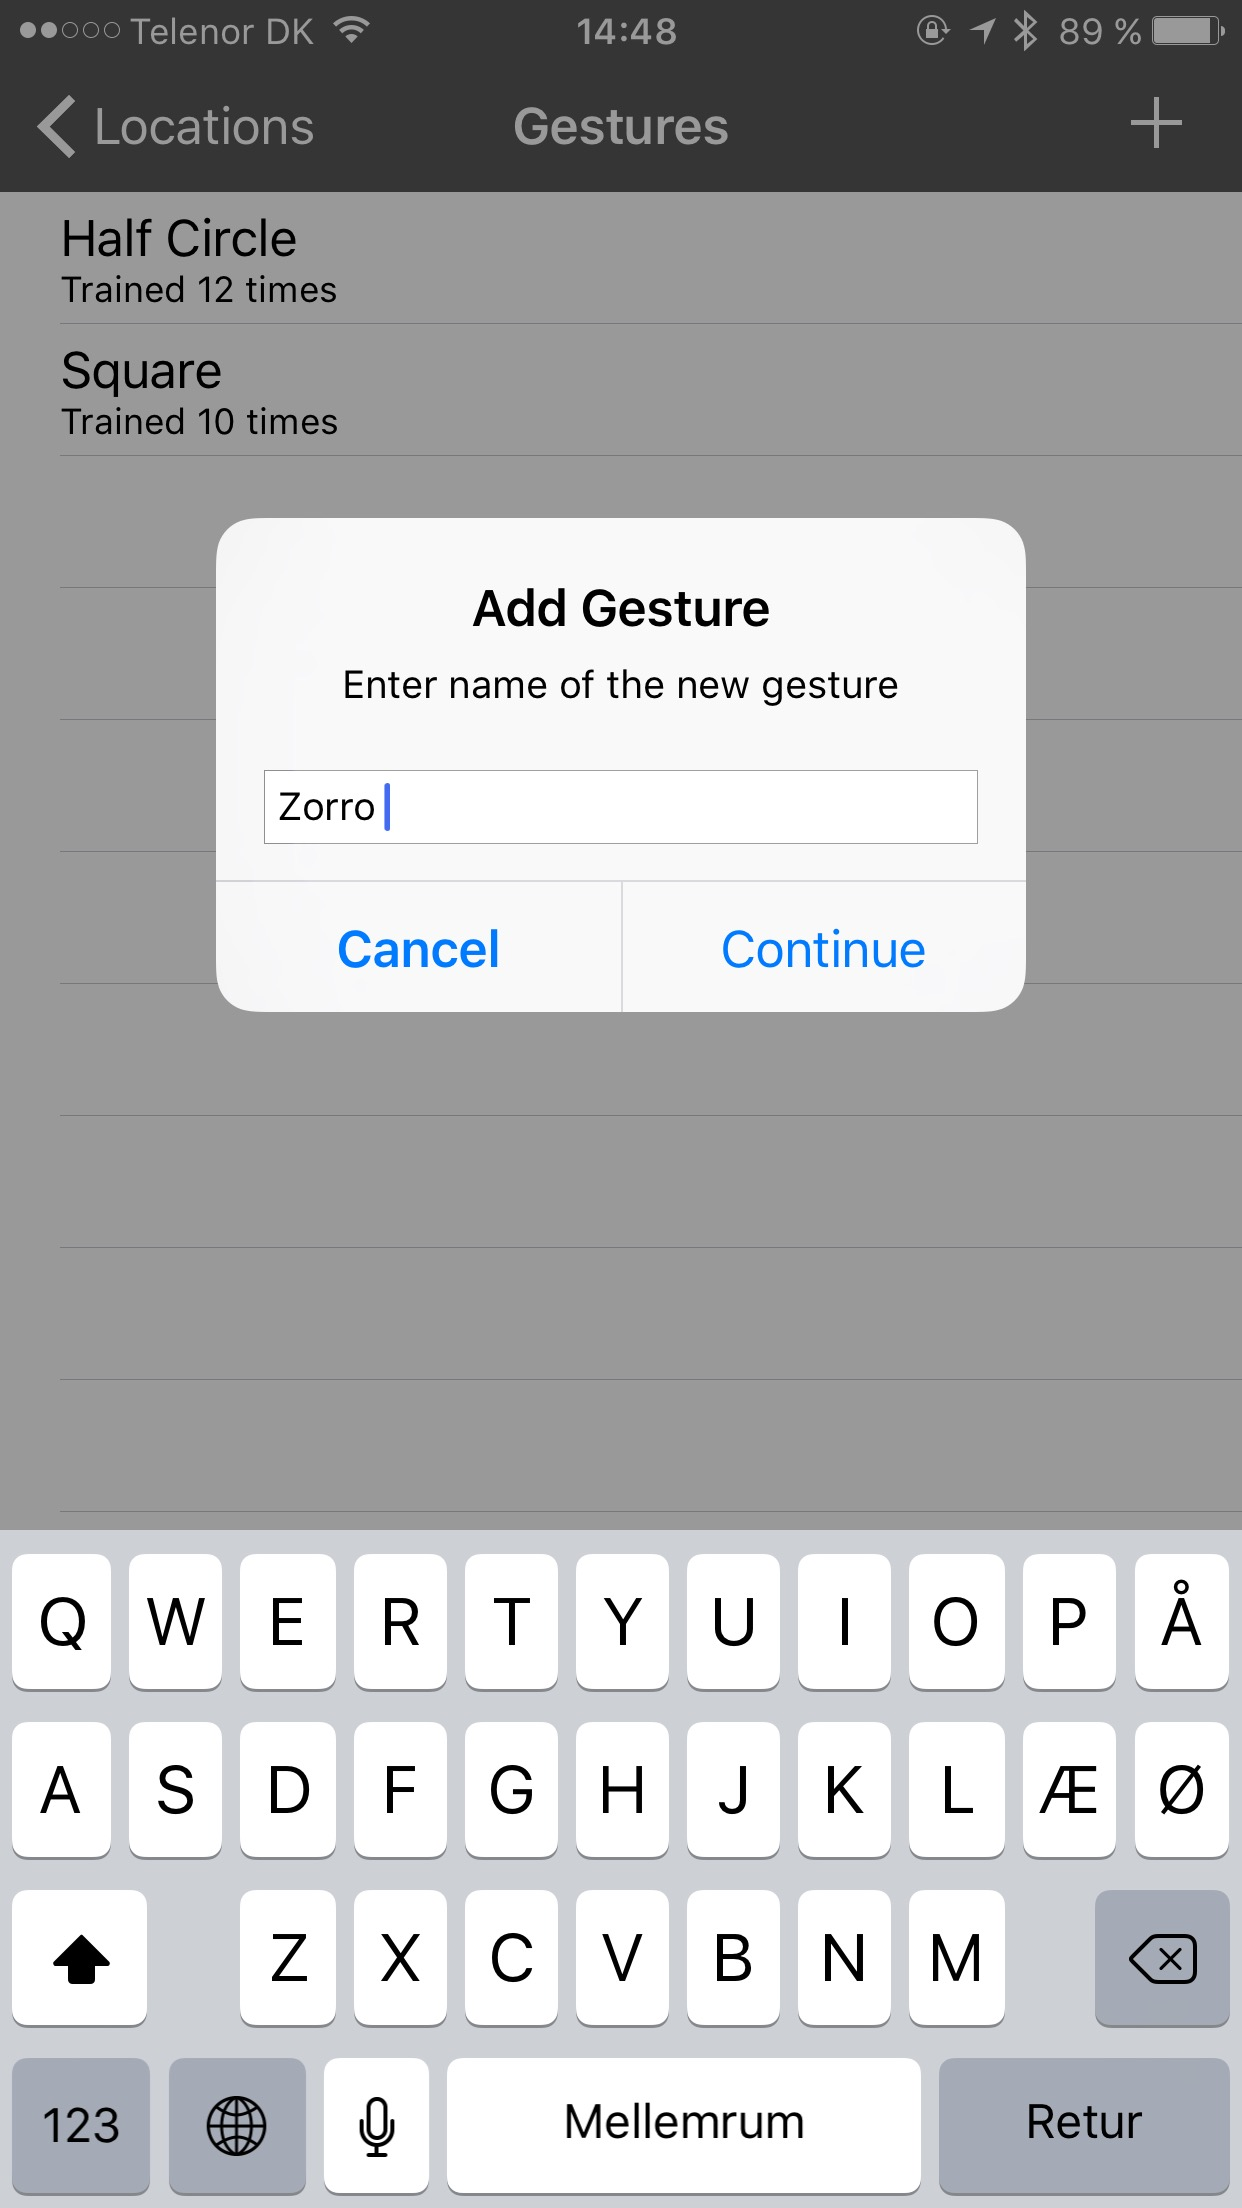
\includegraphics[width=0.3\textwidth]{images/prototype-3-new-gesture}}
    }
    \subfloat{
        \frame{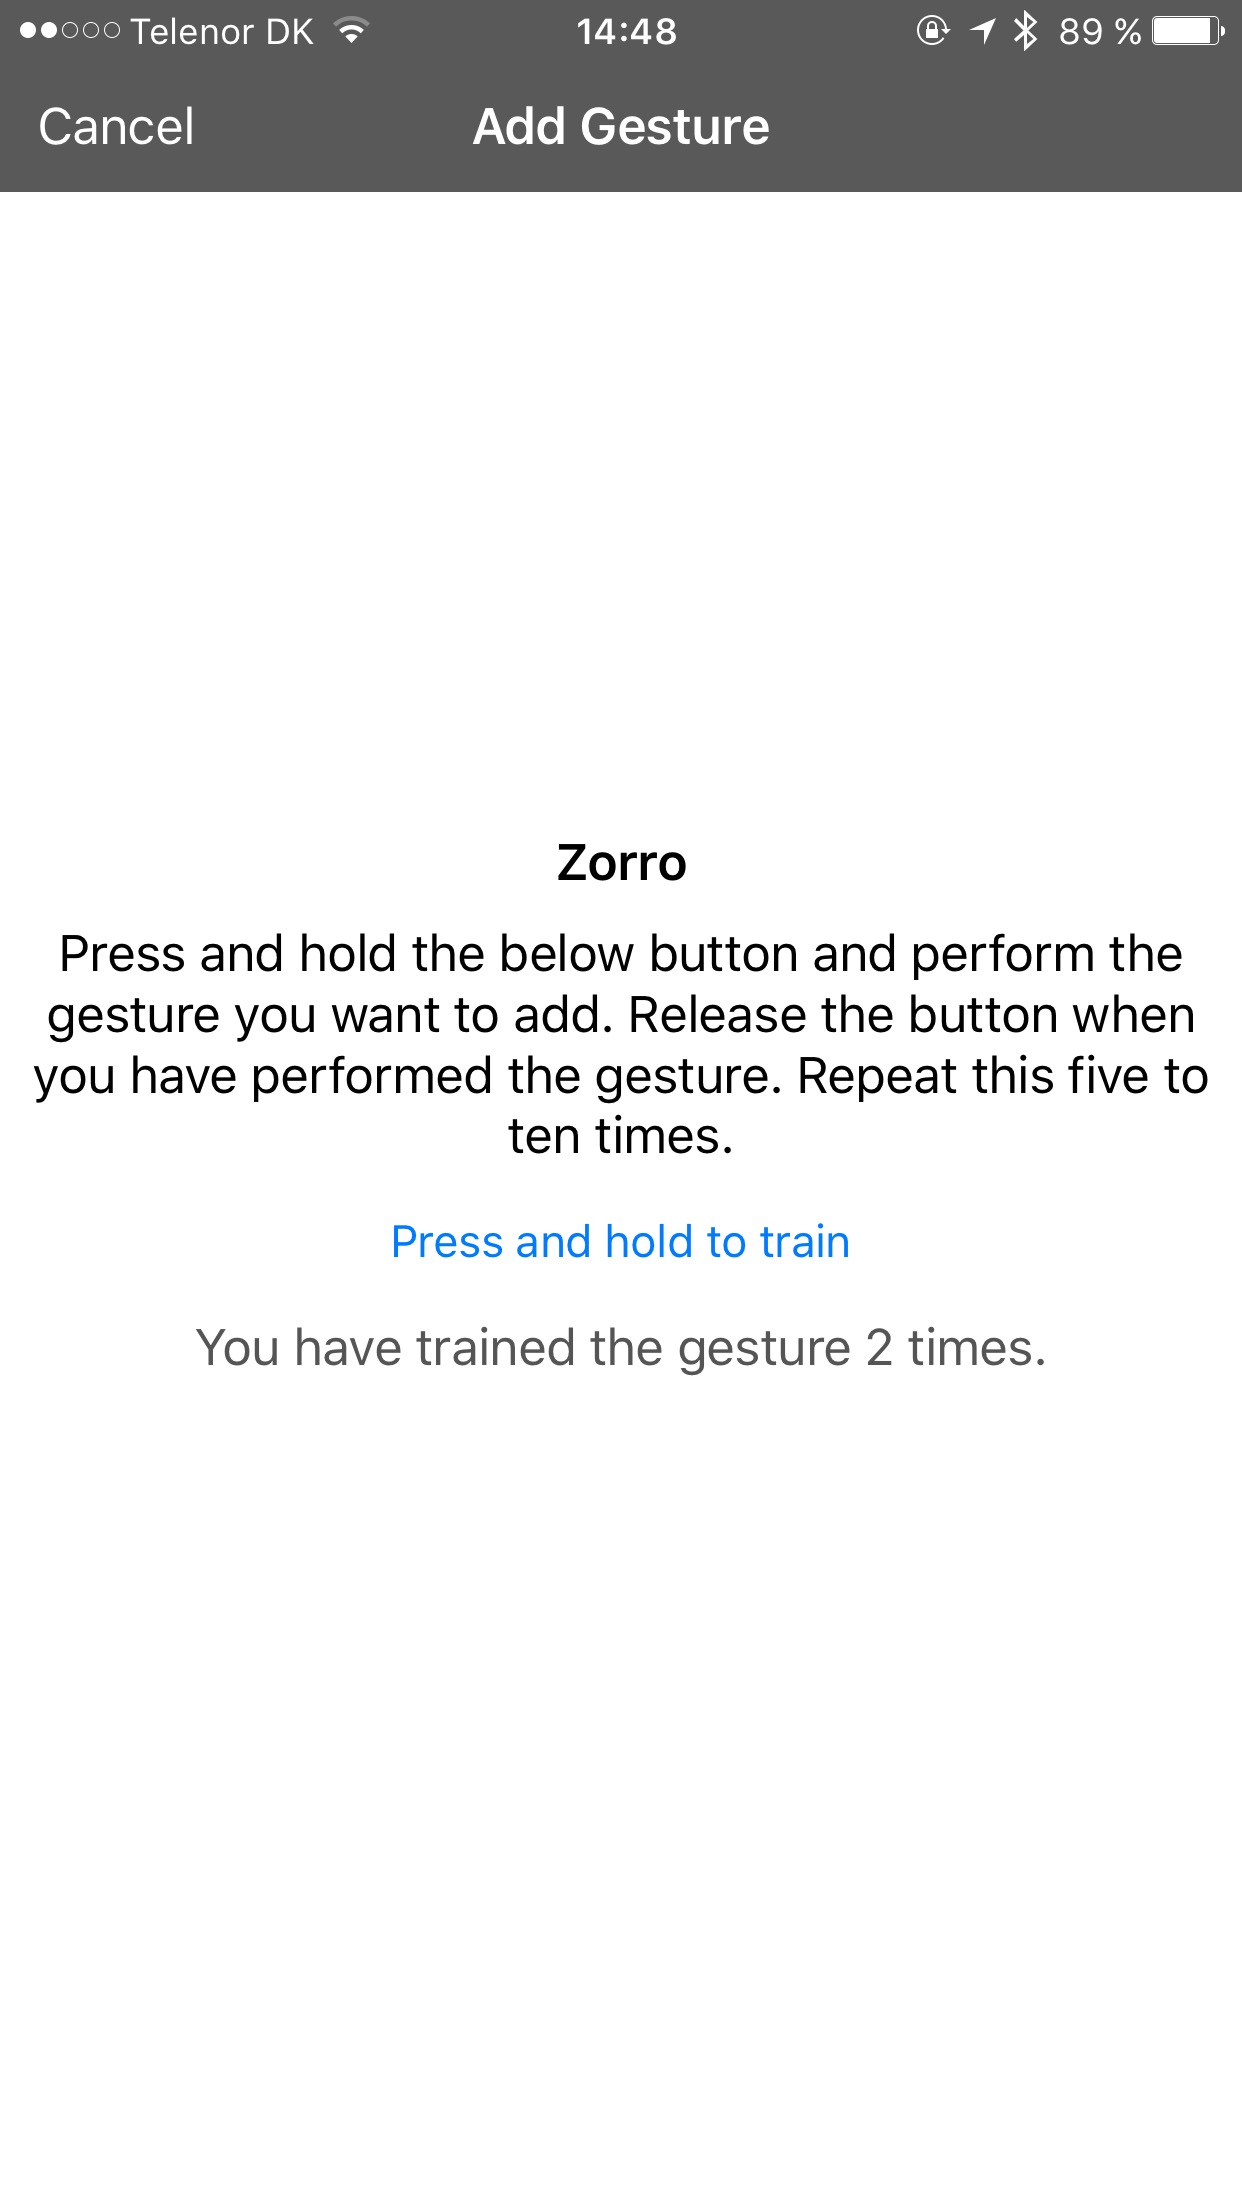
\includegraphics[width=0.3\textwidth]{images/prototype-3-train-gesture}}
    }
    \caption{Screenshots showing the flow and interface for adding and training a new gesture in the third prototype.}
    \label{fig:prototype3-gesture-screenshots}
\end{figure}

\begin{figure}[!htb]%
    \centering
    \frame{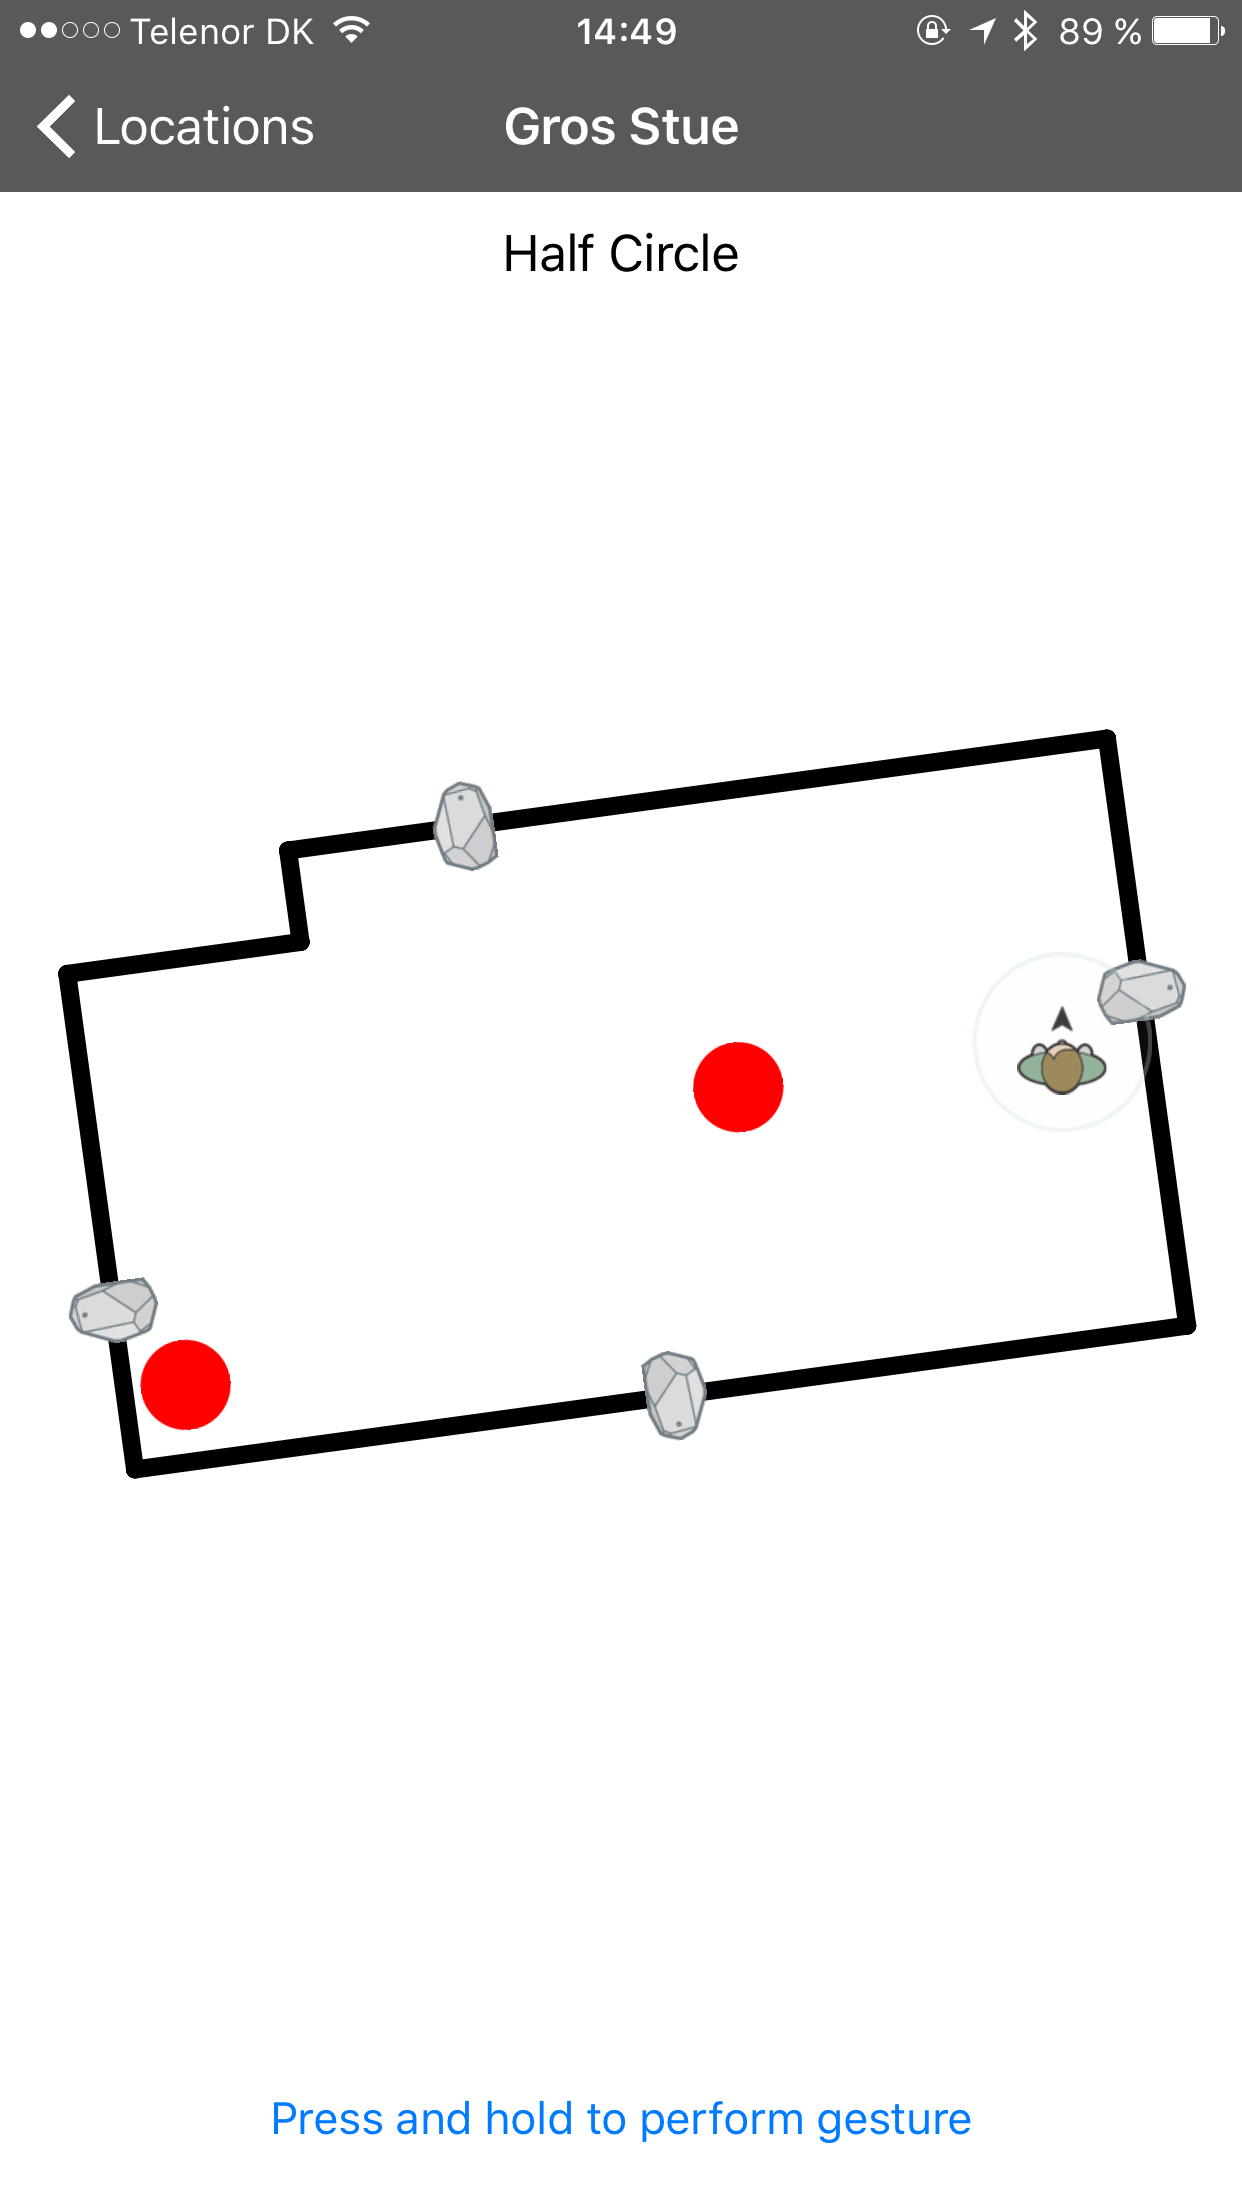
\includegraphics[width=0.3\textwidth]{images/prototype-3-gesture-triggered}}
    \caption{Screenshot showing new representation of the room and controllable devices. In this screenshot the gesture named ``Half Circle'' was recently recognized, and therefore the gesture name is shown in the top of the screen.}
    \label{fig:prototype3-room-screenshot}
\end{figure}

%%% Local Variables:
%%% mode: latex
%%% TeX-master: "../../master"
%%% End:

\FloatBarrier
\section{Final Prototype}
\label{sec:implementation:prototypes:prototype4}
The purpose of the fourth and final prototype of the iOS application, 
was to connect the concepts from previous prototypes, 
into a final prototype and control actual smart devices.

\subsection{Description}
This iteration of the application removed the need for pressing to start and end a gesture. 
Instead the user points with the device, 
in order to select one or more smart devices, 
that should be controlled and perform the gesture, 
after a short delay as described in \Cref{sec:detecting-points}.

Furthermore gestures can be configured per action.
An action is something that a smart device can perform. Actions for a lamp could be \textit{turn on} or \textit{turn off}.

Each action a smart device can perform, 
can be associated with a gesture. 
Several devices can share a single gesture. 
The screenshots in \Cref{fig:prototype4-app-screenshots} shows how this is configured.

The application shows the following four actions:
\begin{itemize}
\item \texttt{turnOn} for the \emph{Lamp at Dinner Table} device
\item \texttt{turnOff} for the \emph{Lamp at Dinner Table} device
\item \texttt{turnOn} for the \emph{Lamp at Couches} device
\item \texttt{turnOff} for the \emph{Lamp at Couches} device
\end{itemize}

Only the first action, 
\texttt{turnOn} for \emph{Lamp at Dinner Table}, 
has a gesture associated with it. 
The three other actions have no gesture configured, 
and therefore cannot be triggered from the application.
In a realistic scenario, all of the actions would have a gesture associated with them.

Tapping on a one of the action/device combinations presents the gesture picker, 
from which gestures can be added or associated with a device and an action. 
Swiping on a action/device combination, 
lets the user remove an associated gesture.

\subsection{Major Changes}

\begin{itemize}
\item Actual smart devices connected to HomePort are controlled, through the server described in \Cref{sec:serverimplementation}.
\item Removed the need for pressing start and stop when performing a gesture. Instead the user points with the smarthpone.
\item Gestures can be associated with a device and action.
\end{itemize}

\subsection{Results}

In the fourth prototype all components were connected, 
and the system could be used as a whole. 
Using the fourth prototype we are able to perform tests on the entire system, 
and get a better understanding of how realistic the initial vision of controlling a smart home, 
by pointing at one ore more devices and perform a gesture, is. 
We are also able to get a better overview, 
of which components of the system need improvements in future work.

The next step could be to fine tune some of the components, 
in order to perform better measured on speed or accuracy or both. 
Another possible step to be taken is to port the solution to wearable.

\begin{figure}[!htb]%
    \centering
    \subfloat{
        \frame{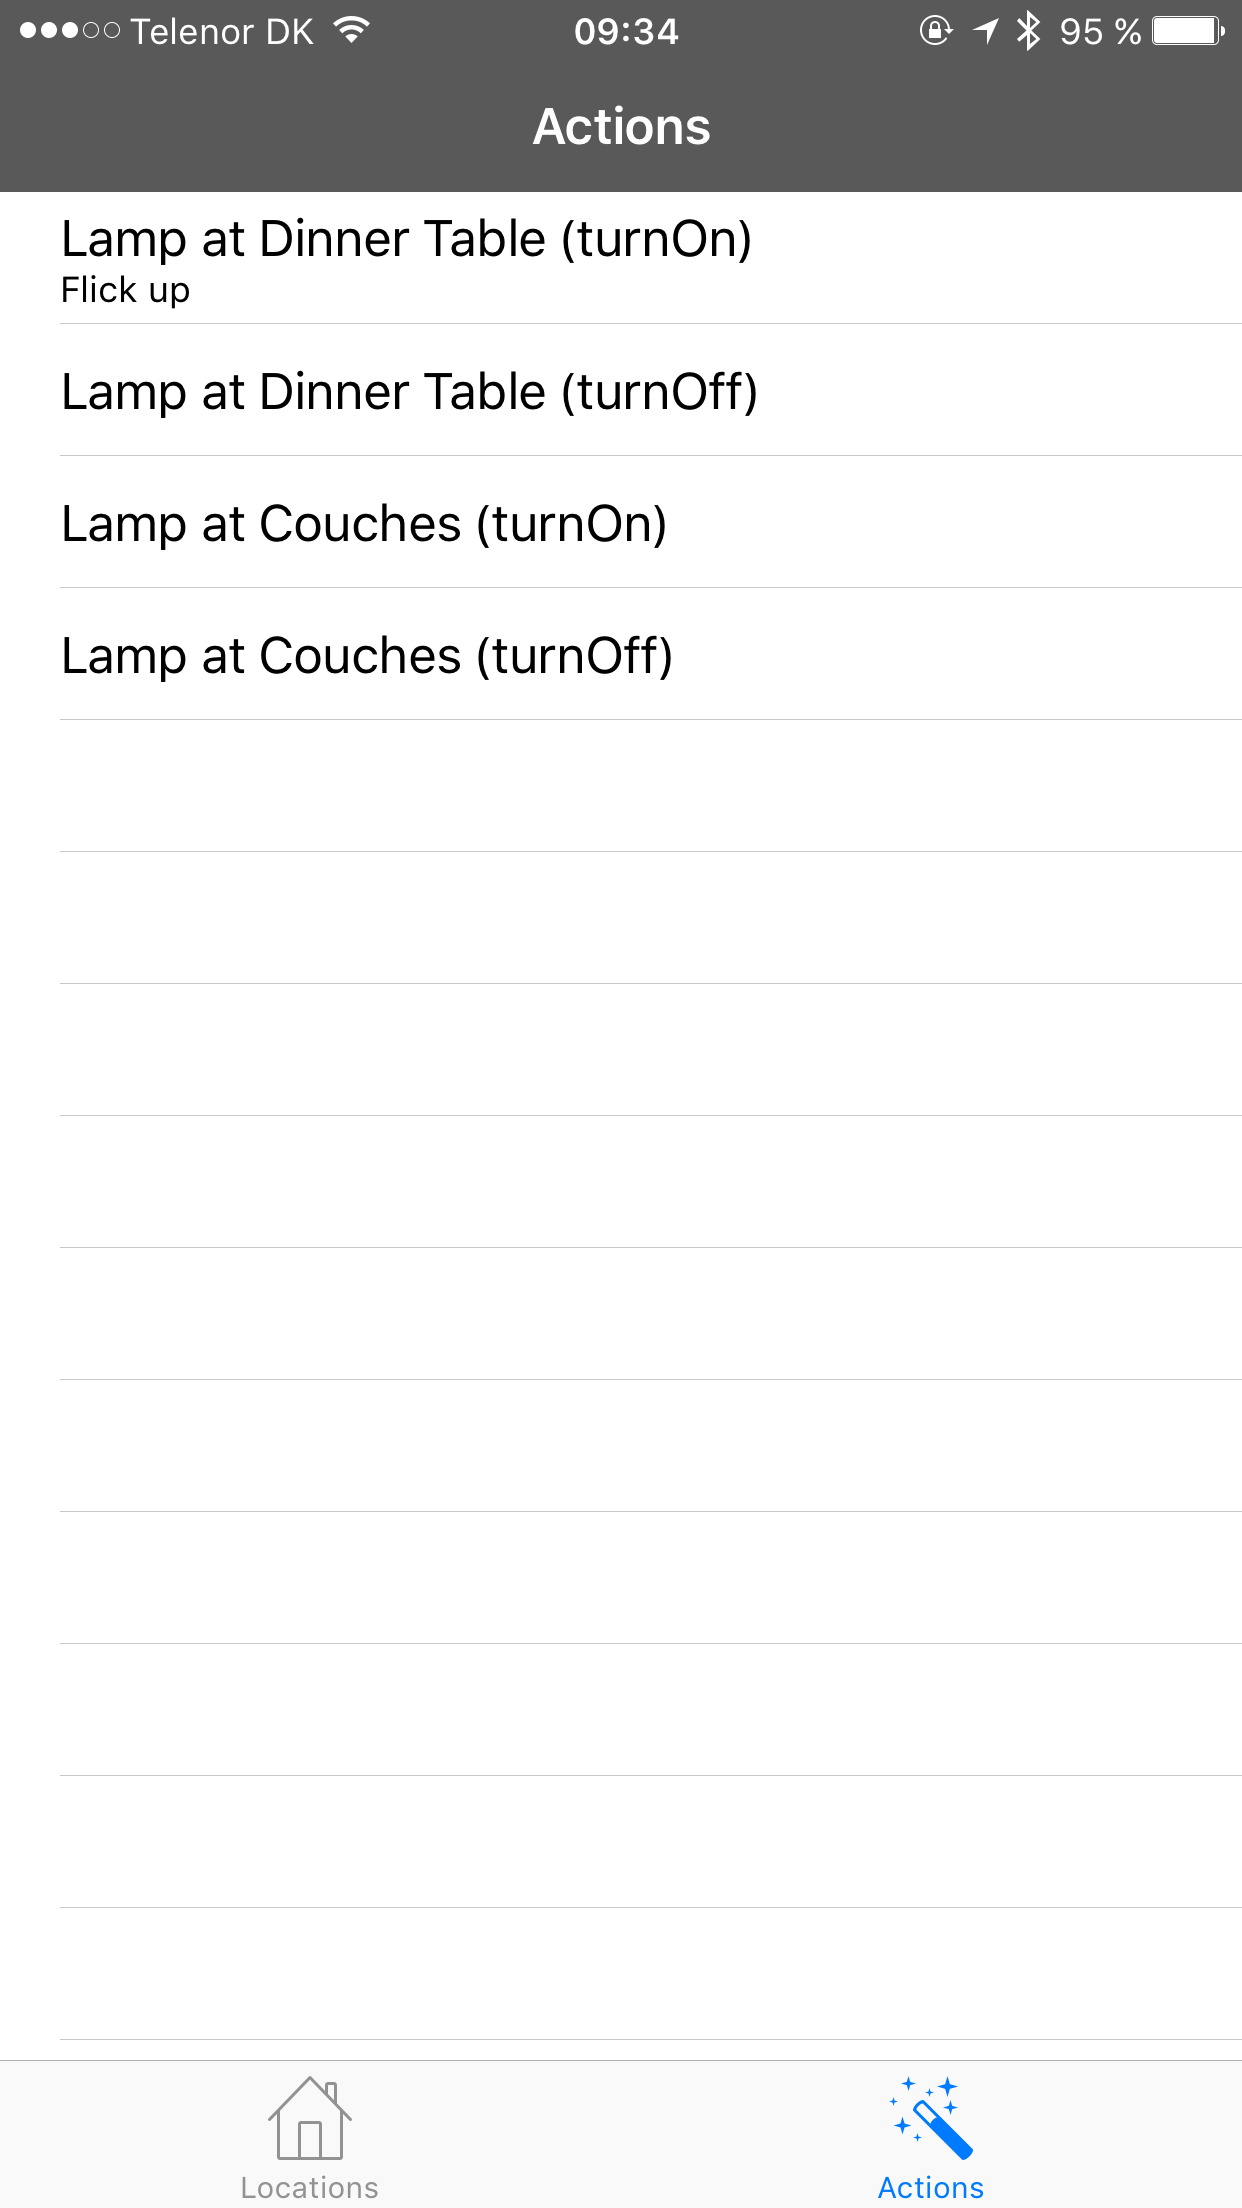
\includegraphics[width=0.3\textwidth]{images/prototype4-1.png}}
    }
    \subfloat{
        \frame{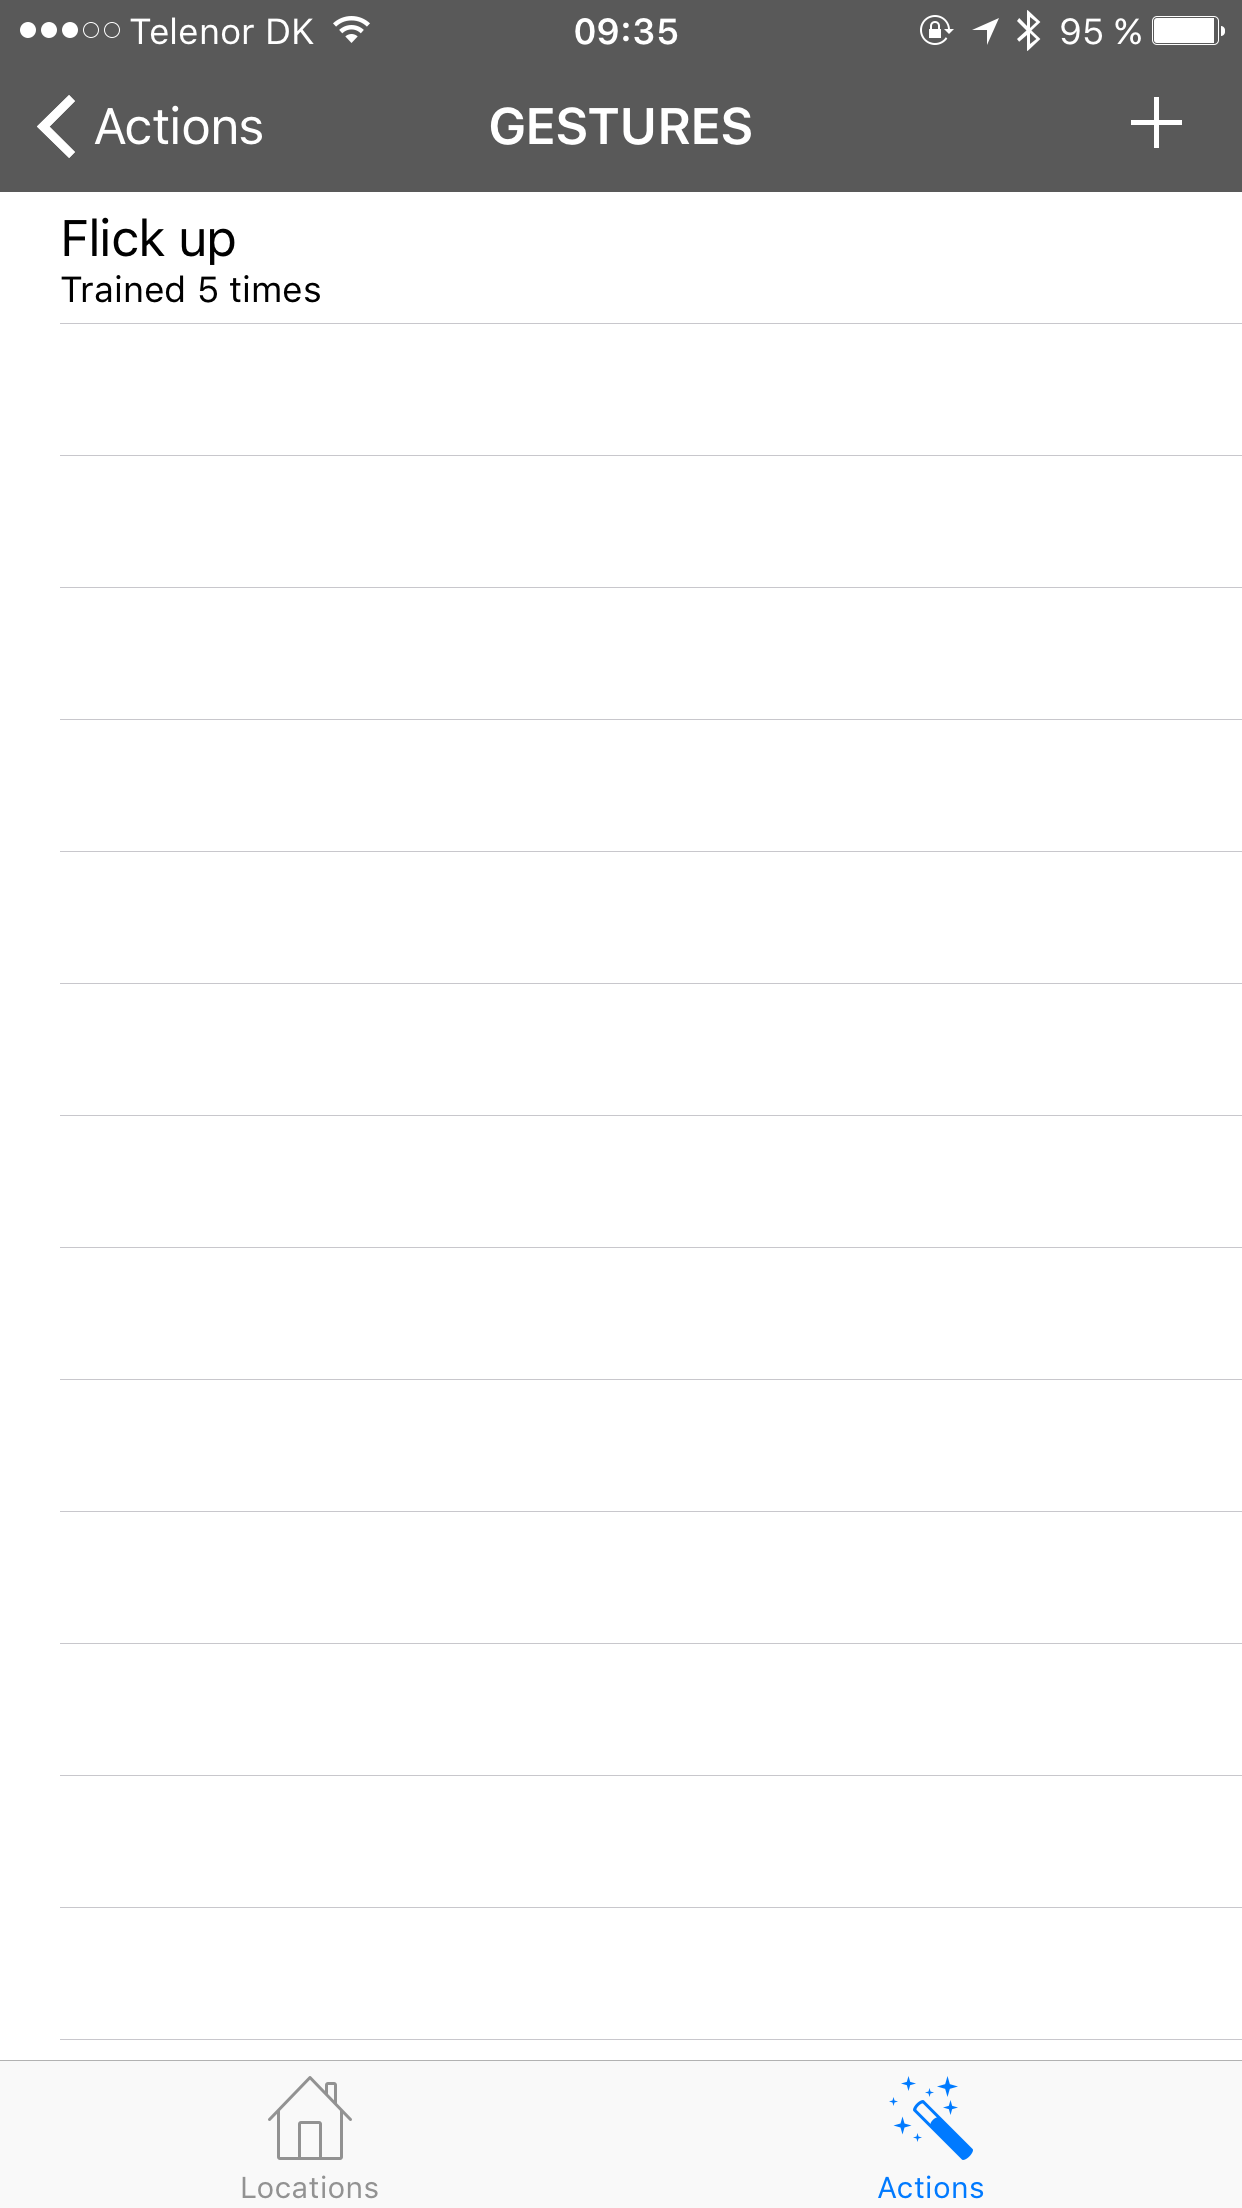
\includegraphics[width=0.3\textwidth]{images/prototype4-2.png}}
    }
    \caption{Screenshots of the fourth and final prototype.}
    \label{fig:prototype4-app-screenshots}
\end{figure}

%%% Local Variables:
%%% mode: latex
%%% TeX-master: "../../master"
%%% End:

\FloatBarrier
\section{Server}\label{sec:serverimplementation}
The server was described in \Cref{sec:serverdesign}. 
In this section, we briefly document the implementation of the server.

The server is implemented in Python,
using a microframework called \texttt{Flask}\footnote{http://flask.pocoo.org/},
which provides a built-in server and a RESTful request handler. 
As described in \Cref{sec:serverdesign}, 
the server only provides two REST methods for controlling a devices and getting the devices. 
Using \texttt{Flask}, the structure of the implementation can be seen in \Cref{lst:server}.

\begin{listing}
  \begin{minted}[linenos, breaklines, autogobble]{python}
    from flask import Flask
    app = Flask(__name__)
    
    @app.route('/', methods=['POST'])
    def do_action():
      action = request.form['action']
      id = request.form['id']
      # Code to send request to HomePort
      
    @app.route('/devices', methods=['GET'])
    def get_devices():
      # Code to return devices from HomePort
    
    if __name__ == '__main__':
    app.run(host="localhost", port=5000)
  \end{minted}
  \caption{Simple server implemented in Python using Flask.}
  \label{lst:server}
\end{listing}

\subsection{Communication with HomePort}
In order to communicate with HomePort, 
we need to do
\begin{enumerate}
  \item Map actions as strings, to actions as numeric values
  \item Send HTTP requests (\texttt{GET} and \texttt{PUT})
  \item Transform XML data from HomePort to JSON
\end{enumerate}

We have borrowed a box from Aalborg University,
containing two ordinary light bulbs, 
a Phidget interface kit and a relay.
This Phidget box has been used to test the implementation of connecting with HomePort. 

\subsubsection{Mapping Actions}
In the current implementation of HomePort, 
there is only two actions: $\{0, 1\}$.
We implement two actions: $\{\var{turnOff}, \var{turnOn}\}$. 
Actions are implemented differently on the server, 
in order to give each action a meaningful value, 
\eg ``turnOn'' is more descriptive than a ``0''.
The two sets of actions are implemented as a list of tuples, 
where the first value is the HomePort value, 
and the second value is our string value. 

To map the actions, we either send a numeric value (map to string) or a string value (map to numeric), 
and look up either the numeric or string value in our list of tuples of actions.

If the list of tuples is
\begin{center}
  \texttt{ACTIONS = [('0', 'turnOff'), ('1', 'turnOn')]},
\end{center}
then if we send \texttt{0}, we get \texttt{'turnOff'}. 

\subsubsection{Sending HTTP Requests}
We use another Python module called httplib, 
to send the requests from the server to HomePort. 
The request we send are either a GET or a PUT. 
The GET is simply a \texttt{GET /devices HTTP/1.1}. 

To perform an action, we use the aforementioned mapper to get the numeric value of our action and send a PUT request with 
\begin{minted}[breaklines, autogobble]{python}
"<?xml version='1.0' encoding='UTF-8'?><value>" + actionID + "</value>"
\end{minted}
as data. 

\subsubsection{Transforming XML Data}
When we request devices from HomePort, 
we receive an XML response. 
An example response of HomePort could be:
\begin{minted}[linenos, breaklines, autogobble, escapeinside=||]{xml}
<?xml version="1.0"?>
<devicelist name="services.xml" id="12345">
  <device desc="phidget" id="173111" vendorid="0x01" productid="0x01" version="V1" location="ExampleRoom" type="phidget">
    ...
    <service desc="input" id="0" value_url="/phidget/173111/output/0" type="input" unit="0/1">
      <parameter id="0"/>
    </service>
    |\ldots|
  </device>
</devicelist>
\end{minted}

The values that we are interested in here are the attributes of the \texttt{service} element, 
mainly the attributes \texttt{id}, \texttt{value\_url} and \texttt{unit}. 
The \texttt{desc} attribute has the potential to contain the name of the smart device, 
but is not so in the version of HomePort that we are using. 
We will use the \texttt{id} to identify the HomePort, 
the \texttt{value\_url} to easily send actions to the device, 
and \texttt{unit} to figure out what actions are available. 

The \texttt{unit} attribute is however not compatible with our actions, 
so we transform the string \texttt{''0/1''} to a list \texttt{['0', '1']}, 
and then use our mapper to convert these to our actions. 

We also need to get the state of the device. 
If we know the state of the device, 
we are able to use a single gesture for on and off,
\ie the action of the gesture could simply switch the binary state of the device. 
In HomePort, the state is either 0 (off) or 1 (on). 
To get the state of the device, 
we can do a \texttt{GET} request to the URL of the device, \eg:
\begin{center}
  \texttt{GET /phidget/173111/output/0},
\end{center}
and then map the state of HomePort to our states.

The names and coordinates of the \texttt{Device} objects must be inserted by the user and are currently hardcoded, 
as we have not implemented adding new devices. 

The JSON result of the transformed XML, with a name and coordinate is:

\begin{minted}[linenos, breaklines, autogobble, escapeinside=||]{xml}
{
  "devices": [
  {
    "actions": ["turnOff", "turnOn"], 
    "coords": [6.5, 3.35], 
    "id": "0", 
    "name": "Lamp at Couches", 
    "state": "off", 
    "url": "/phidget/173111/output/0"
  }, 
  {|\ldots|}
  ]
}
\end{minted}
